\section{実験結果と考察}

\subsection{βスズ試料の作成}
空間的に一様にできたのは試料1、2、3、6だった。

\subsubsection{βスズ試料のX線回折による構造分析}
$\rm 2\theta/\theta$配置において室温でAs grown試料のX線回折強度を測定し、試料の構造解析を行った。基板には多結晶のガラスを用いた。

図\ref{fig:intensity_asgrown_samples}に、試料1、2、3、6の回折強度を$2\theta$に対してプロットしたものを示す。また空間群の対称性をもつβスズの室温での(293K)での格子定数a=b=5.8303 Aとc=3.1810A \cite{Wolcyrz}から、粉末X線回折スペクトルを再現した図も併せて示す(Reference)。
\begin{figure}[!h]
    \begin{center}
   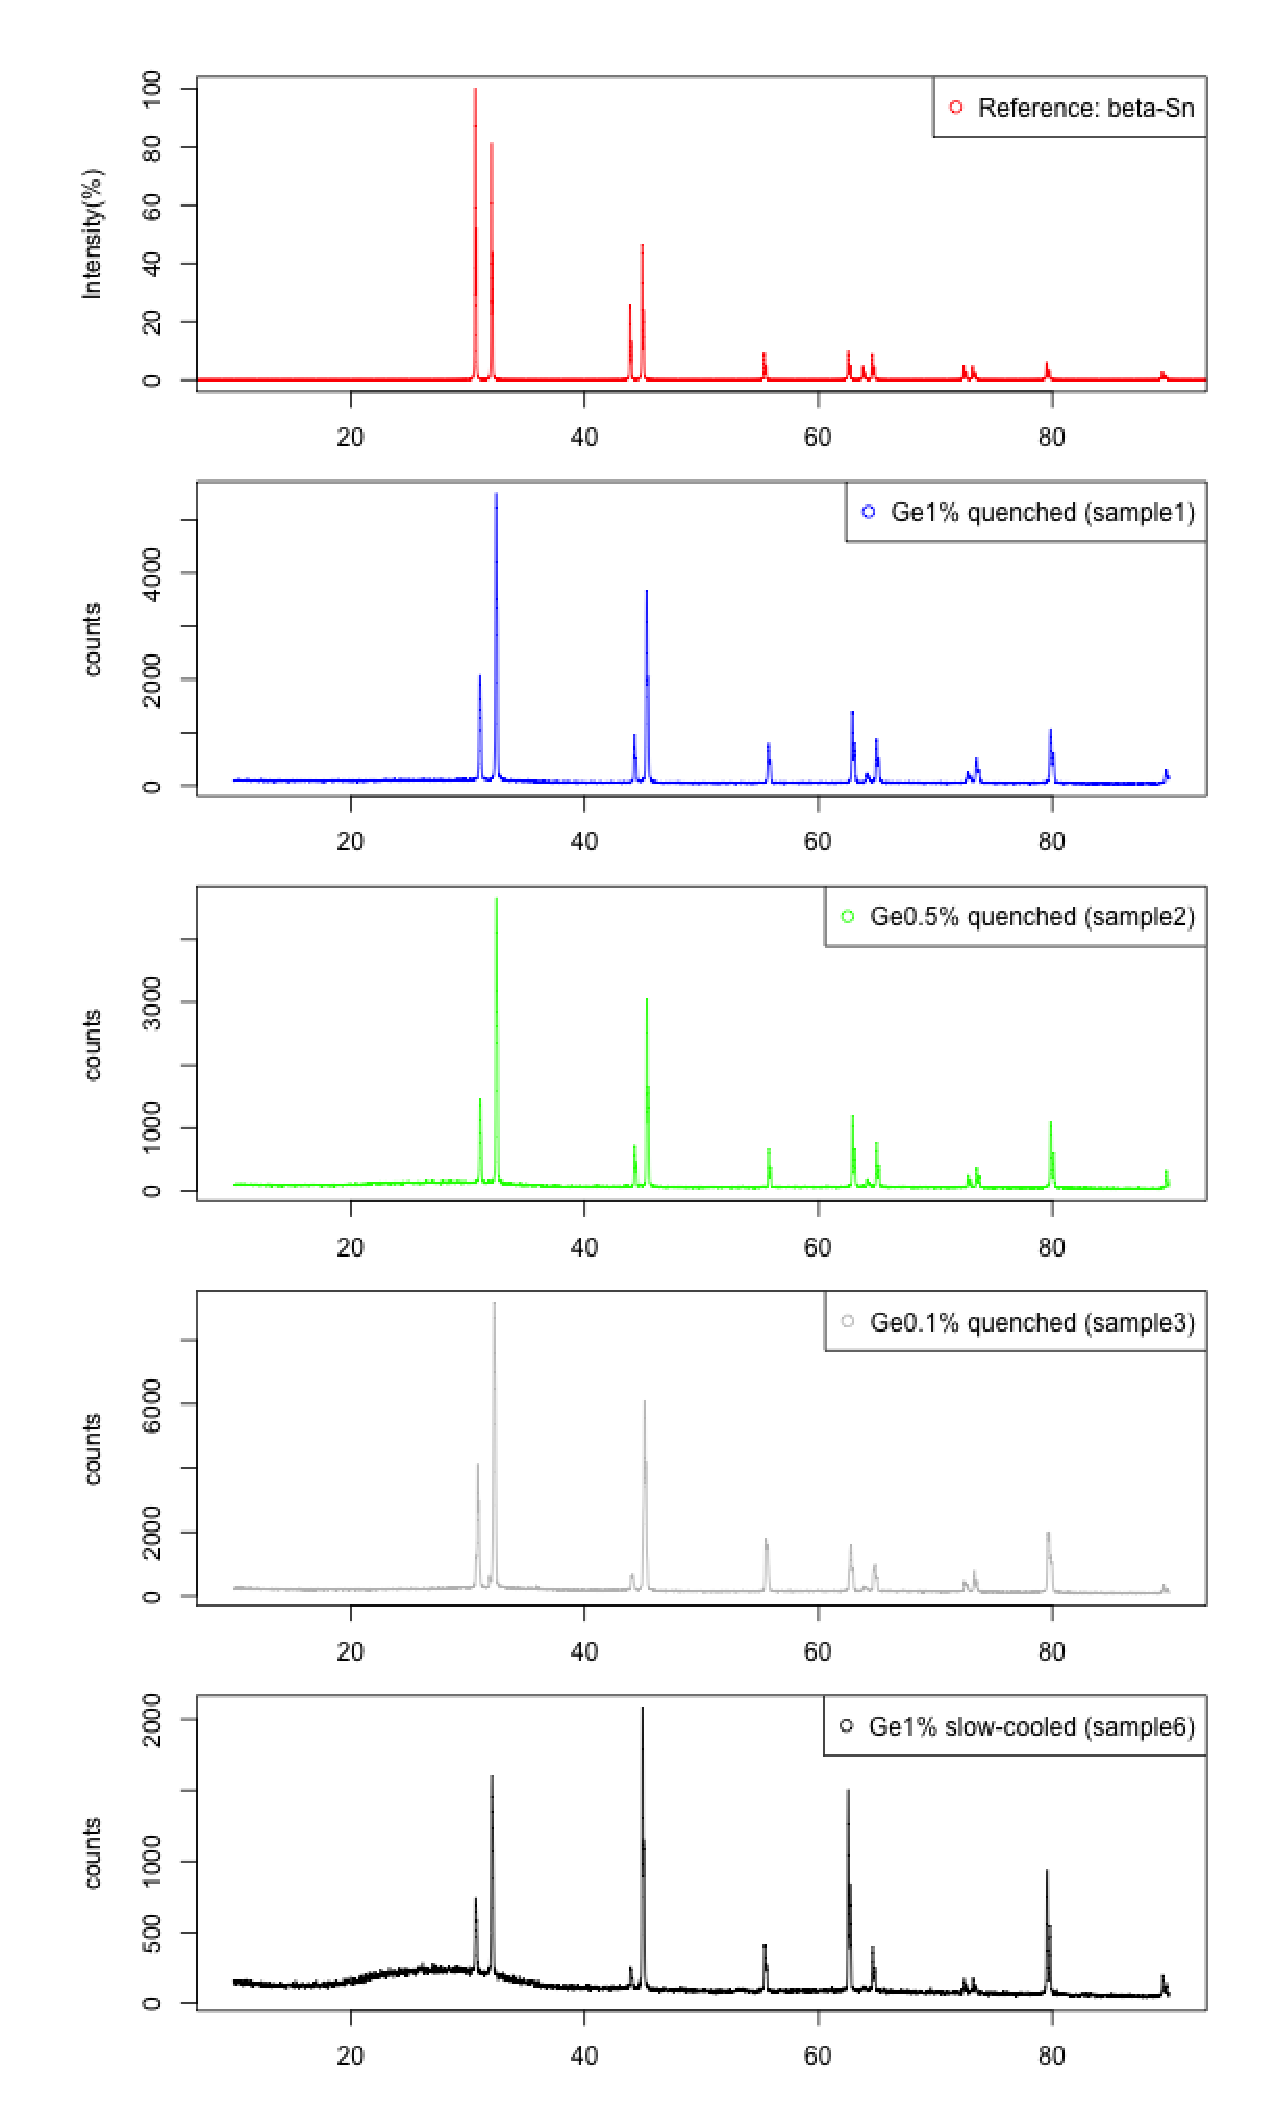
\includegraphics[width=0.8\hsize]{results_discussions/intensity_asgrown_samples.eps}
  \end{center}
  \caption{As grown(β相)試料}
  \label{fig:intensity_asgrown_samples}
\end{figure}

それぞれの試料に対して、βスズの粉末X線回折で現れる全てのピークが見えている。すなわち、試料はそれぞれβスズと同一の構造を持った多結晶を含むことが分かる。またGeやαスズに由来する回折のピークは見られず、大部分がβスズであることを確かめた。なお試料6において、$2\theta=20^\circ$から$2\theta=40^\circ$にかけて、ブロードな回折が見られる。これはアモルファス構造を持つ石英ガラスのハロー回折である\cite{Speakman}。しかしこのブロードなスペクトルの影響は小さいため無視できる。

\subsection{αスズ試料への変換}
表\ref{tab:trans_Time}に、βスズからαスズへの転移にかかった時間をまとめる。
As grownの試料2(Ge0.5 wt. \% /急冷)と試料3(Ge0.1 wt. \% /急冷)は数日から一週間程度の時間スケールで相転移が完了した。一方、試料1(Ge1 wt. \% /急冷)は数週間程度の時間スケールで相転移が進行しなかった。

そこでまず筆者は試料1では何らかの理由でαスズの核が生成されていないのではないかと仮説を立てた。核生成は試料の内部より表面やエッジから始まりやすい\cite{Cornelius}ため、α相からβ相への相転移にかかる時間は傷をつけた試料の方がAs grown試料より始まりやすい。実際、筆者は相転移が進行している最中の試料を観察することで、エッジから核生成がなされていることを確認した。筆者は試料1の表面にカッターナイフで傷を入れたり、ニッパーで切り込みを入れることで各生成を促進しようとした。しかしそのような工夫をしても、数週間程度の時間スケールで相転移は進行しなかった。

そのサンプルを3ヶ月間ほど家庭用冷蔵庫の冷凍室の中に放置しておくと、相転移が完了していることを確認した。Matvienkoらの研究によるとβスズのαスズへの転移はβスズの塑性変形が重要な役割を果たすが、その塑性変形とそれに伴う欠陥の拡散をβスズ中に分散したGeが阻害するため、Geの添加はαスズへの転移速度を遅くする\cite{Matvienko}(図\ref{fig:Ge_content})。これからGeをGe1 wt. \%添加した試料1の相転移が非常に遅く、相転移を観察できなかったことと筆者は考える。

一方、試料1と同様にGeをGe1 wt. \% 添加した試料6(Ge1 wt. \% /徐冷)は数日程度の時間スケールで相転移が完了した。これは溶融試料を冷却する際、試料1を10秒程度の時間スケールで水クエンチ(急冷)したのに対し試料6は48時間かけて徐冷したことによる、冷却速度の違いによるものであると筆者は考える。Ge-Sn合金の平衡相図を表した図\ref{fig:GeSn_phase}とそのGeリッチ領域を拡大した図\ref{fig:GeSn_phase2}によると、99wt. \%スズ-1 wt. \%Ge(99at. \%スズ-1at. \%Ge)合金は、冷却に330℃程度でスズを1.1at.\%程度固溶したGeを晶出し、その結果Sn-Ge溶液のGe濃度は共出点のGe濃度0.3 at. \%程度\cite{Thurmond1960}まで落ち込む。その濃度でさらに共晶反応が起こり、Snリッチな領域とGeリッチな領域に分離する。したがって冷却時に部分的に平衡状態にあったと仮定するなら、試料6のSnリッチな領域はGe濃度が1 wt/\%より低くなっている。また試料6は冷却にかけた時間が平衡状態を保つのに不十分で偏析しているとしても、部分的にGeリッチな領域が晶出または析出して、Snリッチな領域のGe濃度が1 wt/\%より低くなっているとする結論は変わらない。
一方、10秒程度の時間スケールでの急冷で相分離は起こらない(要出典/EdX)。したがって試料1においてGe濃度は空間的に一様である。
\begin{table}[!h]
    \begin{center}
  \begin{tabular}{c|ccccc}
    & 試料1(Ge1\%/急冷) & 試料2(Ge0.5\%/急冷) & 試料3 (Ge0.1\%/急冷)& 試料5(Ge1\%/400℃まで加熱/急冷) & 試料6(Ge1\%/急冷) \\ \hline
    As grown & 1ヶ月以上3ヶ月以内 & 1週間以内 & 1週間以内 & 1週間以内 & 数日 \\
  \end{tabular}
  \caption{β相からα相への転移にかかる時間(電気炉により加熱した試料)}
  \label{tab:trans_Time}
    \end{center}
\end{table}

\begin{table}[!h]
    \begin{center}
  \begin{tabular}{c|ccc}
    & 試料11(Ge1\%/放冷) & 試料12(Ge0.1\%/放冷) & 試料13(Ge0\%/放冷) \\ \hline
    As grown & 2週間以内 & 2週間以内 & 2週間以上 \\
  \end{tabular}
  \caption{β相からα相への転移にかかる時間(により加熱した試料)}
  \label{tab:trans_Time}
    \end{center}
\end{table}

\subsubsection{αスズ試料のX線回折による構造分析}
$\rm 2\theta/\theta$配置において室温でαスズに変換された試料のX線回折強度を測定し、試料の構造解析を行った。αスズの試料は割れていて小さいので固定が難しく、基板の上に置くと出っ張ってしまう。そこで炭酸カルシウムを主成分とする粘土に埋め込み、平らな上にしてX線を入射した。

%図\ref{fig:intensity_pested_samples}に、試料2、3の回折強度を$2\theta$に対してプロットしたものを示す。なお示したのは、測定された強度からリファレンスとして測定した炭酸カルシウムの強度(CaCO3)を単純に減じた値の正の部分である。また空間群$$の対称性をもつαスズの室温での(293K)での格子定数a=b=c=6.4892\AA \cite{THEWLIS}から、粉末X線回折スペクトルを再現した図も併せて示す(alpha-Sn)。
\begin{figure}[!h]
  \begin{center}
  \includegraphics[width=0.8\hsize]{results_discussions/intensity_pested_samples.eps}
  \end{center}
  \caption{α相に変換された試料}
  \label{fig:intensity_pested_samples}
\end{figure}

それぞれの試料の回折強度には、αスズまたは炭酸カルシウムに由来するピークが現れている。したがって冷凍庫に保持した後、as grown試料には見られなかったαスズが現れたことが分かる。またGeやβスズに由来する回折のピークは見られないため、大部分がαスズであることが言える。

回折強度がところどころが負になっている理由は、主に二つあると筆者は考える。一つ目はリファレンスの強度が適正な値より大きくなっていることである。試料を取り外し炭酸カルシウム粘土のレフェレンスを測定する際、試料が覆っていたところにもX線が入射する。したがって試料以外からの寄与は大きく見積もられる。二つ目は試料の高さがわずかに変化した影響である。この効果はリファレンスを引き算するとき、影響が大きい。
回折角$\rm 2\theta$しかしこれらの問題点は、冷凍庫で保持した後のスズのうちがαスズの構造が支配的であるとする筆者の結論に影響を与えない。


\subsection{α相からβ相への転移温度}
作成後、家庭用冷蔵庫の冷凍室に保持しα相に変換した試料に関して、加熱しながら抵抗測定を行ったところ、ある温度以上で抵抗が大きく落ち込んだ。試料2、3、6の抵抗の温度依存性を図\ref{fig:Trans}に、試料の抵抗の温度依存性を図\ref{fig:Trans}に示す。またその試料の温度を下げてゆくと温度が小さくなるにつれて温度に対し線形に抵抗が減少した。試料の抵抗が落ち込みはじめた温度とで、半導体のα相から金属のβ相への相転移が起きた。
\begin{figure}[!h]
 \begin{minipage}{\hsize}
    \begin{center}
   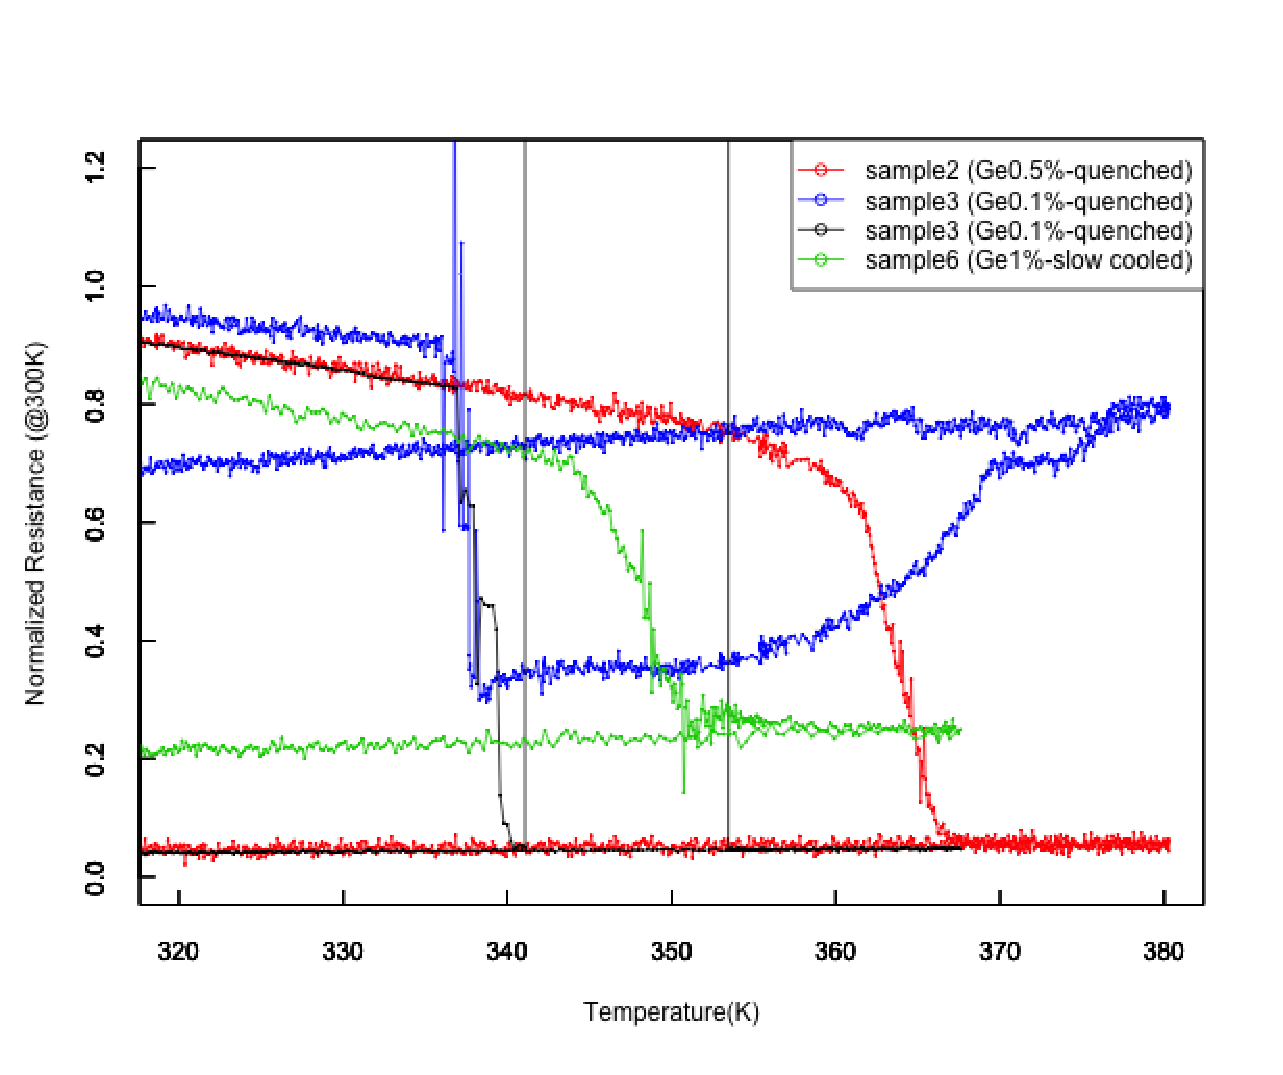
\includegraphics[width=0.9\hsize]{results_discussions/Trans.eps}
  \end{center}
  \caption{}
  \label{fig:Trans}
 \end{minipage}
 \begin{minipage}{\hsize}
     \begin{center}
   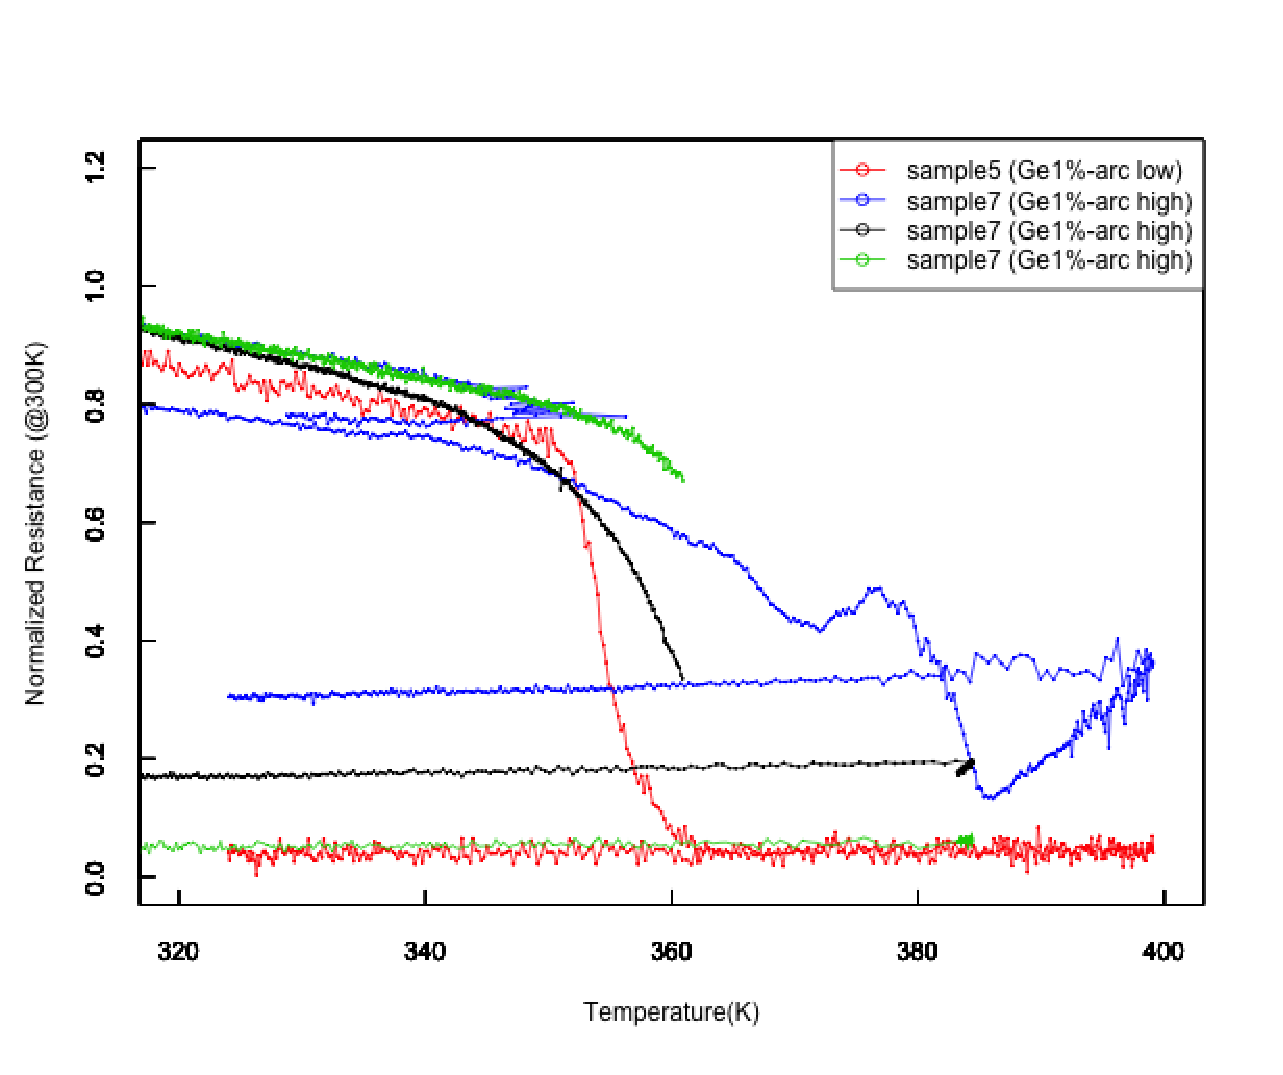
\includegraphics[width=0.9\hsize]{results_discussions/Trans2.eps}
  \end{center}
  \caption{}
  \label{fig:Trans2}
   \end{minipage}
\end{figure}

表\ref{tab:transT}に見積もった相転移温度を示し、図\ref{fig:TransitionT}に相転移を示す。
\begin{table}[!h]
  \begin{center}
  \begin{tabular}{c|ccc}
    & 試料2(Ge0.5\%/急冷) & 試料3(Ge0.1\%/急冷)& 試料6(Ge1\%/徐冷) \\ \hline
     転移が始まる温度(K)& 362 & 337 & 344 \\
     転移温度(K)               & 364 & 338.5 & 347 \\
     転移が終わる温度(K)& 267  & 341 & 351     \\
  \end{tabular}
  \caption{一様な試料がα相からβ相へ転移する温度 (転移温度は、抵抗が転移の始まりと終わりの中間値をとる温度)}
  \label{tab:transT}
    \end{center}
\end{table}
\begin{figure}[!h]
    \begin{center}
   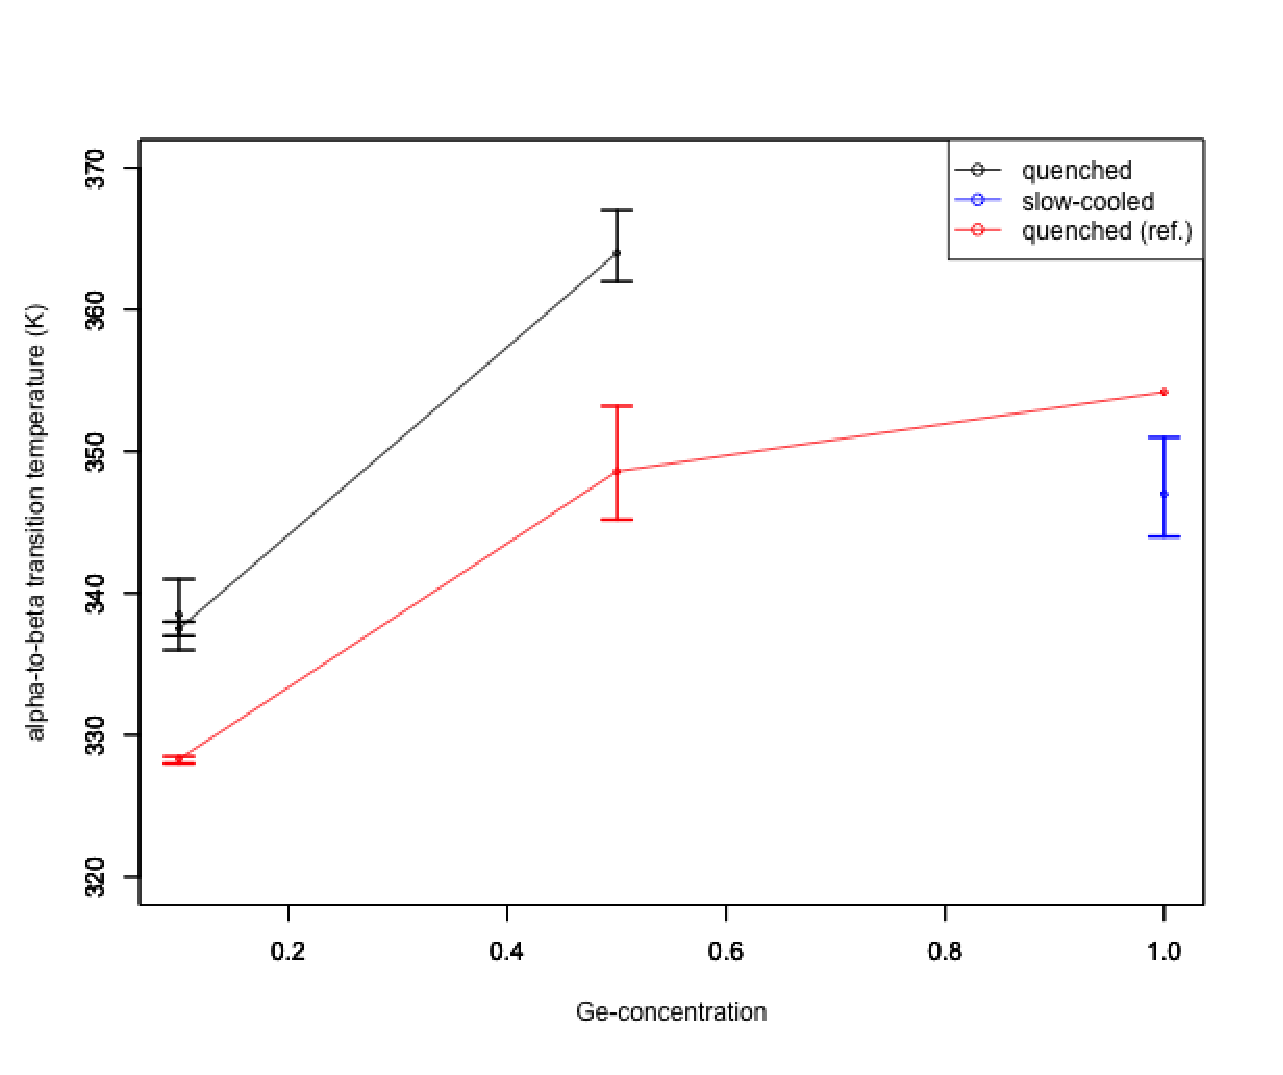
\includegraphics[width=0.9\hsize]{results_discussions/TransitionT.eps}
  \end{center}
  \caption{α相からβ相への転移温度(一様な試料)}
  \label{fig:TransitionT}
\end{figure}



試料2、3、6について、抵抗が変化し始める温度と抵抗の変化が終わる温度、抵抗が始まりと終わりの中間値をとる温度をそれぞれ表に示す。また先行研究によって得られている値と比較して
\begin{table}[!h]
  \begin{center}
  \begin{tabular}{ccc}
    & 試料5(Ge1\%/急冷) & 試料7(Ge0.1\%/急冷)\\ \hline
     転移が始まる温度(K)& &  \\
     転移温度(K)& &  \\
     転移が終わる温度(K)&  &  \\
  \end{tabular}
  \caption{非一様な試料の一部がα相からβ相へ転移する温度 (転移温度は、抵抗が転移の始まりと終わりの中間値をとる温度)}
  \label{tab:transT}
    \end{center}
\end{table}

\begin{table}[!h]
    \begin{center}
  \begin{tabular}{ccc}
    Ge1\%/急冷 & Ge0.5\%/急冷 & Ge0.1\%/急冷  \\ \hline
    $328.3\pm0.3$ & $346.6\pm4.0$ & $354.2\pm0.1$ \\
  \end{tabular}
  \caption{α相からβ相への転移温度(先行研究\cite{})}
  \label{tab:transT_ref}
    \end{center}
\end{table}

\subsection{電流パルスを用いたα相からβ相への変換}
図\ref{fig:181228_before_after_pulse_log}に電流パルス印加前後の抵抗値を示す。パルス印加前(赤色)の抵抗は温度を小さくしながら測定したもので、温度が小さくなるほど抵抗が小さく、半導体的な温度-抵抗依存性を示す。

一方、パルス印加後の抵抗(青色)は60Kより低温で温度が小さくなっていることがわかる。この領域で金属からの寄与が大きく、超伝導体転移が確認できた。

では金属との並列として理解できる\cite{Mayr,McLachlan}

\begin{figure}[!h]
 \begin{minipage}{\hsize}
    \begin{center}
   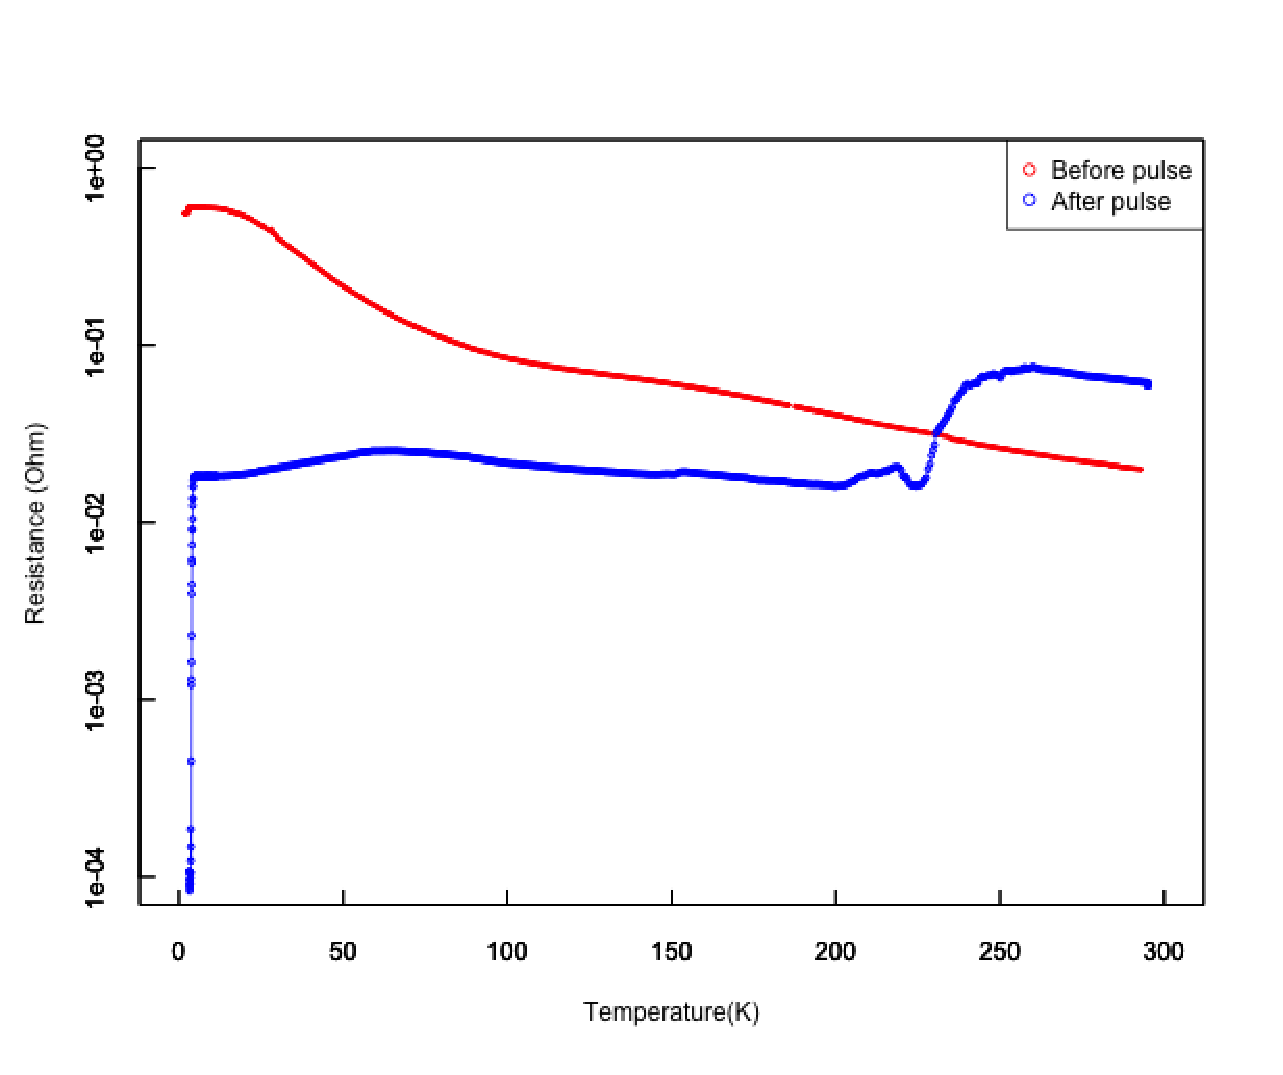
\includegraphics[width=\hsize]{results_discussions/181228_before_after_pulse_log.eps}
  \end{center}
  \caption{}
  \label{fig:181228_before_after_pulse_log}
   \end{minipage}
 \begin{minipage}{0.5\hsize}
    \begin{center}
   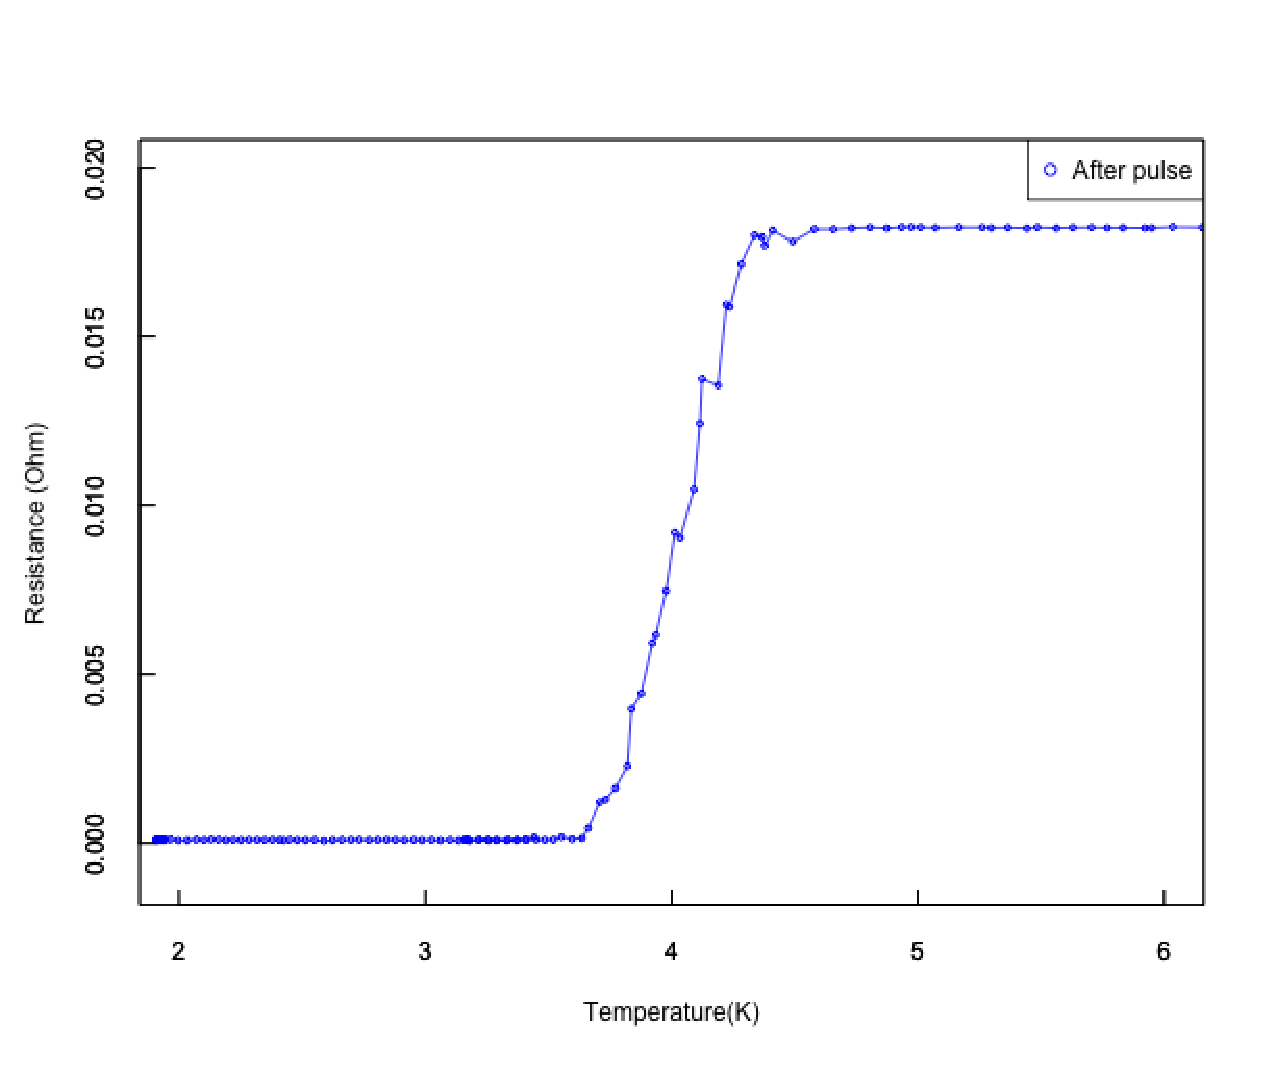
\includegraphics[width=\hsize]{results_discussions/181228_after_pulse.eps}
  \end{center}
  \caption{}
  \label{fig:181228_after_pulse}
 \end{minipage}
 \begin{minipage}{0.5\hsize}
     \begin{center}
   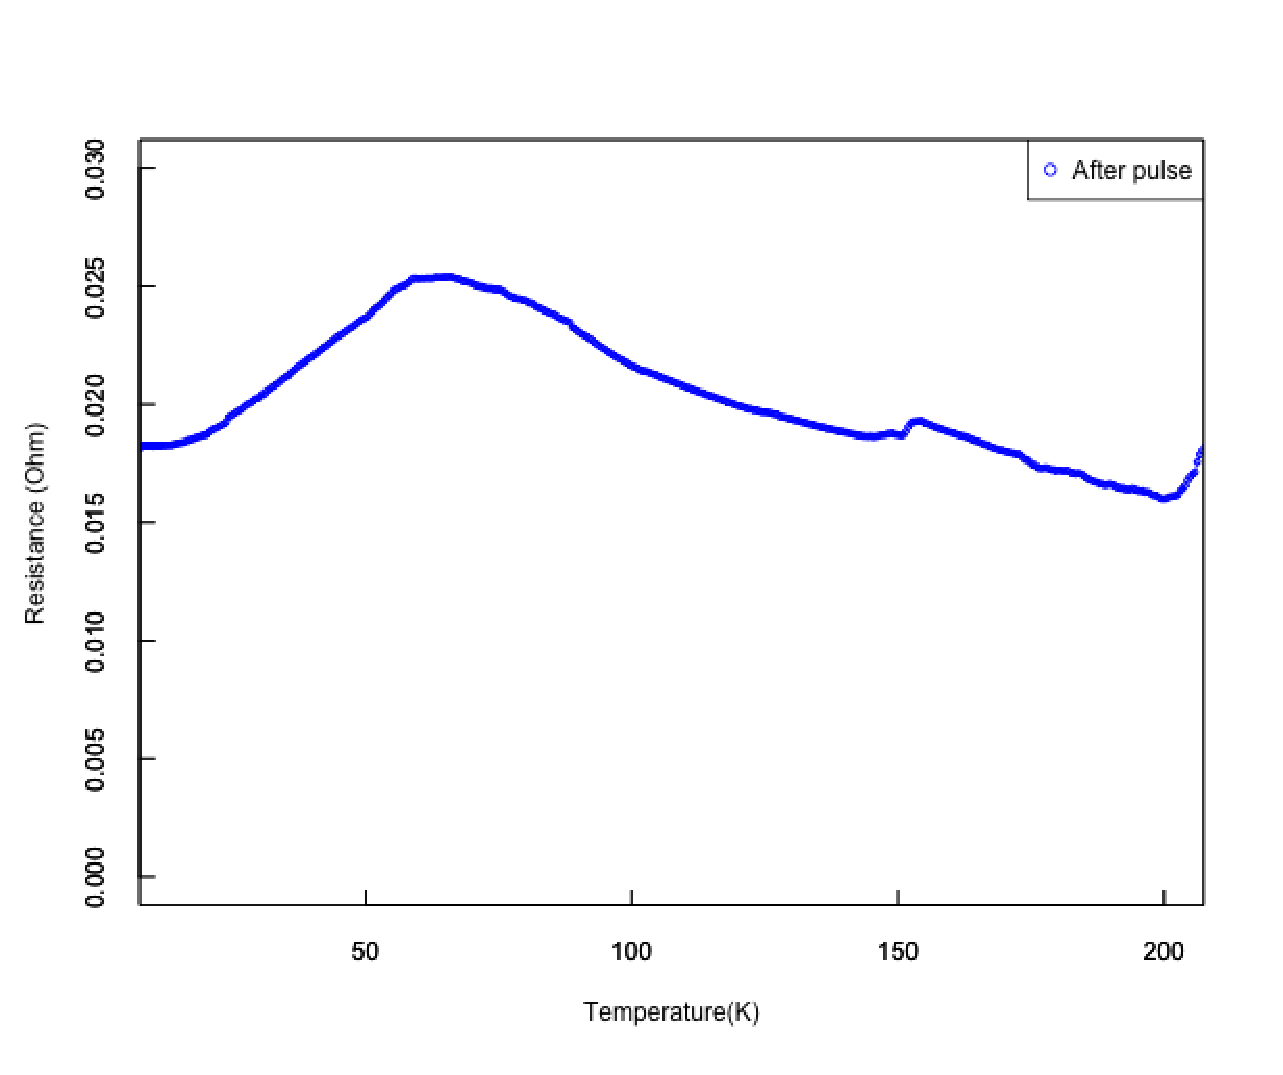
\includegraphics[width=\hsize]{results_discussions/181228_after_pulse2.eps}
  \end{center}
  \caption{}
  \label{fig:181228_after_pulse2}
   \end{minipage}
\end{figure}


\begin{figure}[!h]
 \begin{minipage}{\hsize}
    \begin{center}
   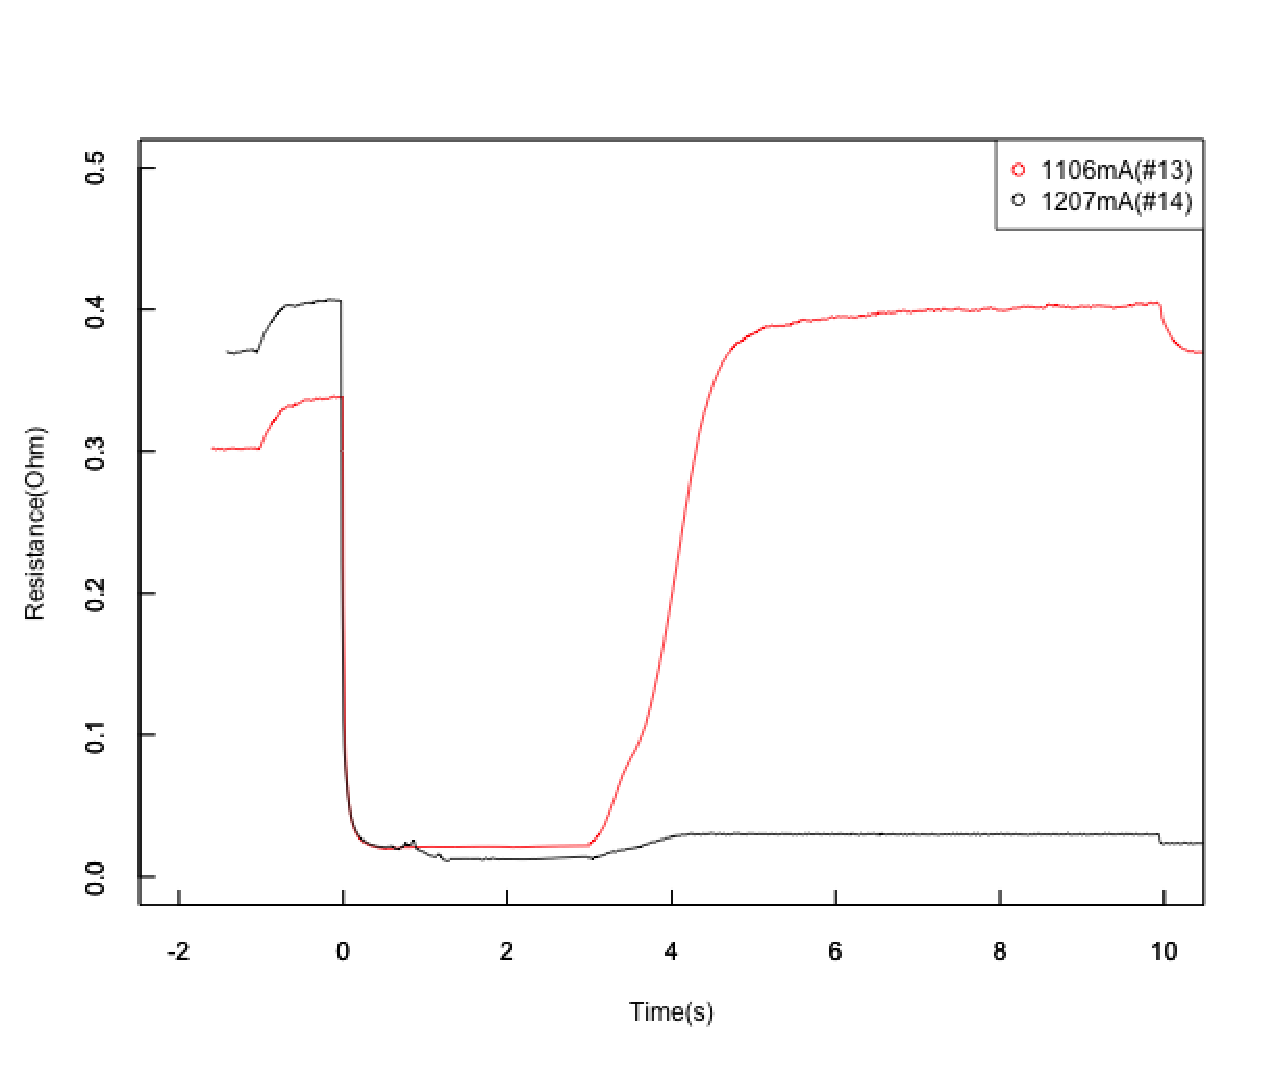
\includegraphics[width=0.7\hsize]{results_discussions/181228_Resistance_pulse_selected.eps}
  \end{center}
  \caption{}
  \label{fig:181228_Resistance_pulse_selected}
 \end{minipage}
 \begin{minipage}{\hsize}
     \begin{center}
   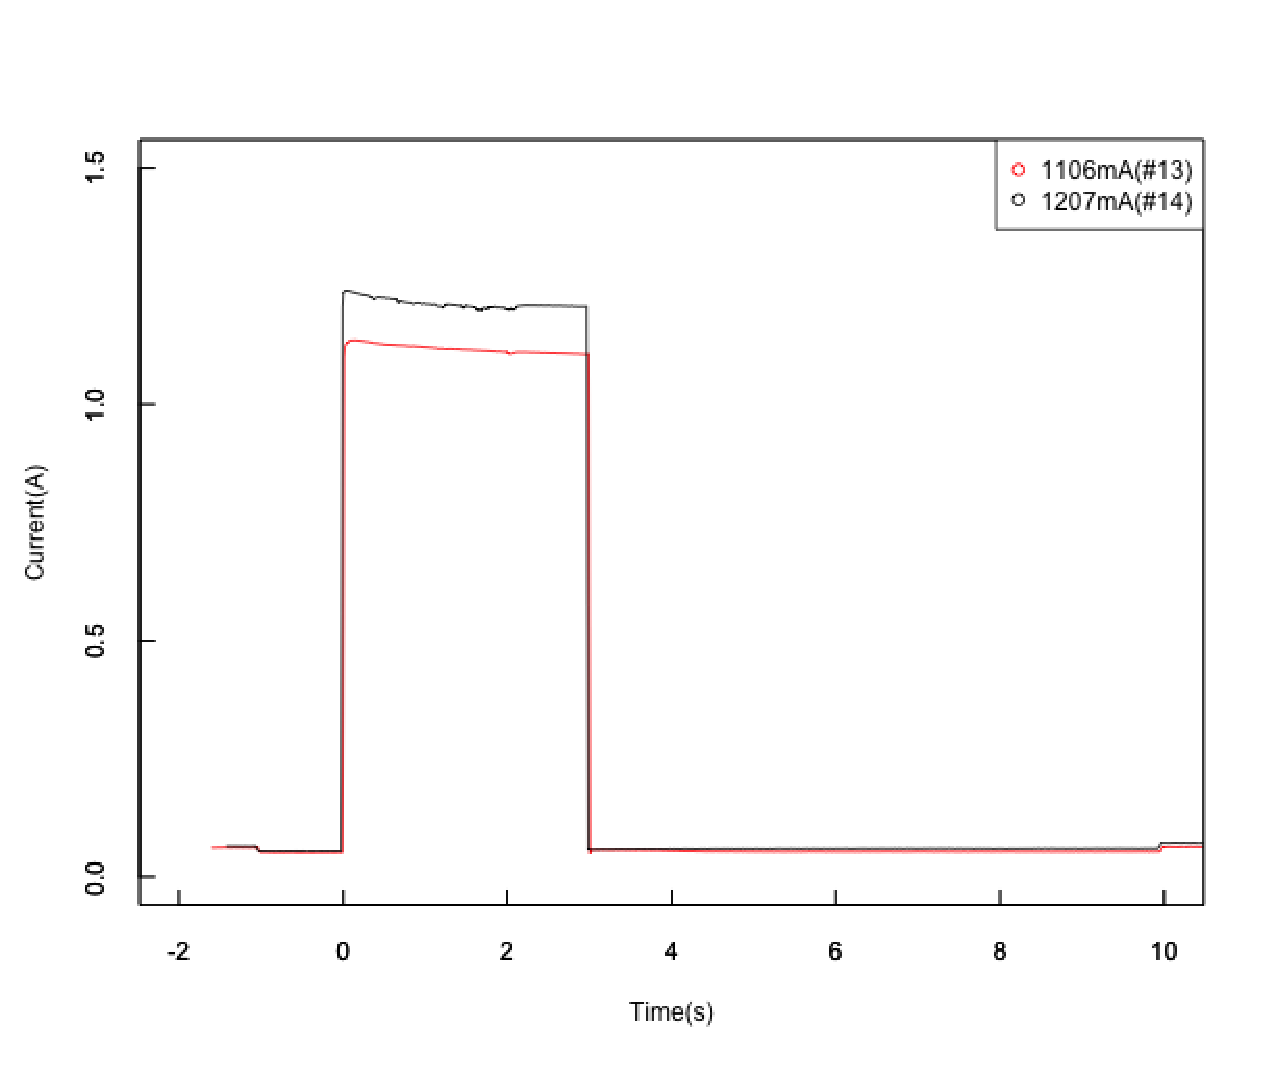
\includegraphics[width=0.7\hsize]{results_discussions/181228_current_pulse_selected.eps}
  \end{center}
  \caption{}
  \label{fig:181228_current_pulse_selected}
   \end{minipage}
\end{figure}

\subsection{電流パルスによるα相とβ相の共存状態の生成}
\begin{figure}[!h]
 \begin{minipage}{\hsize}
    \begin{center}
   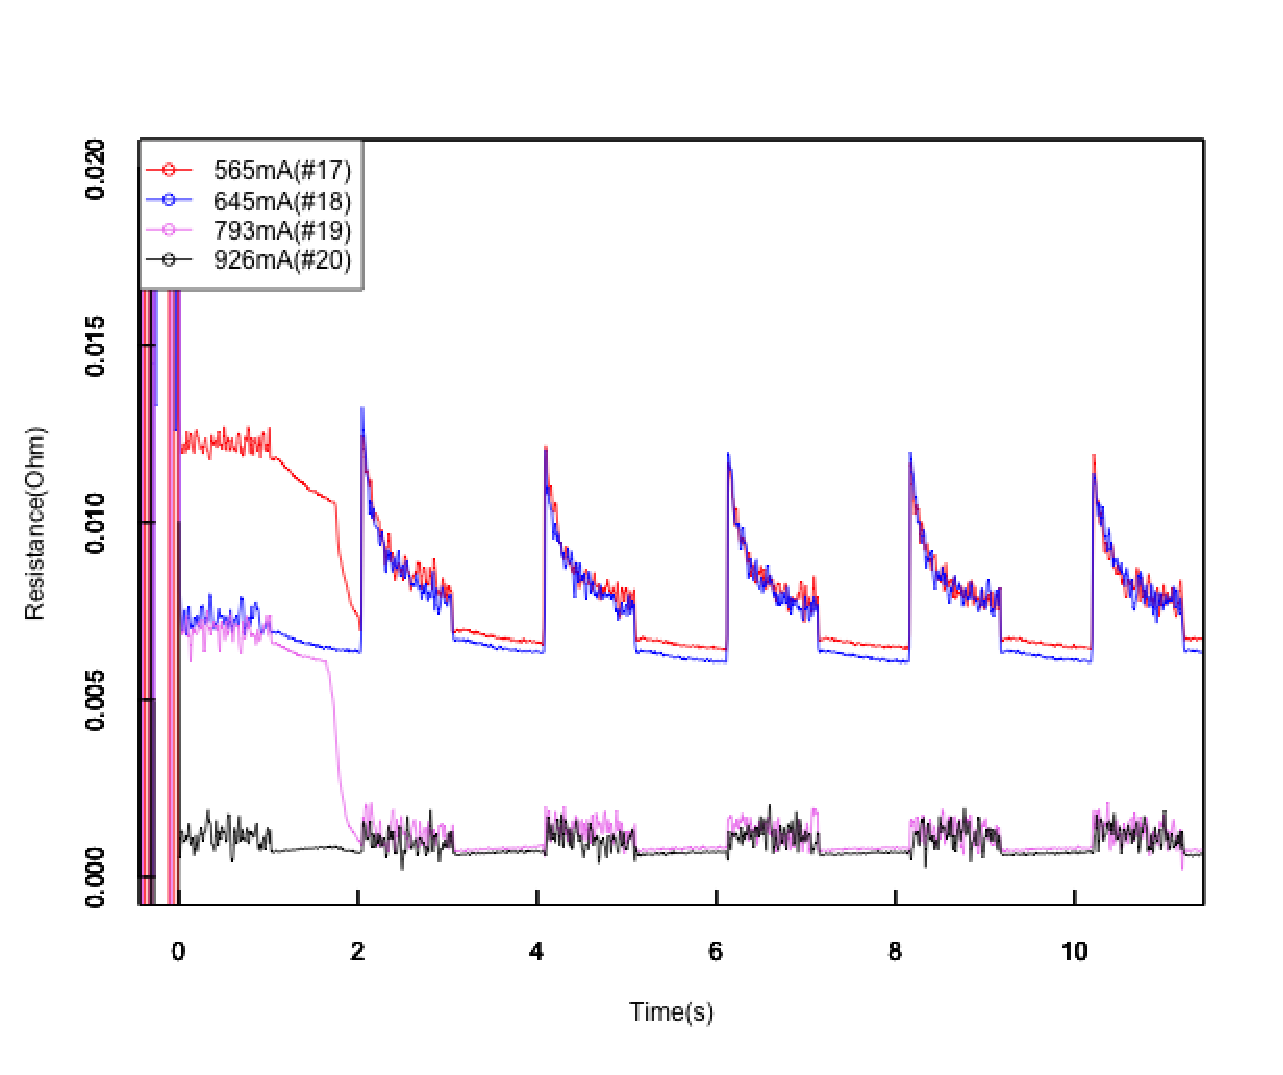
\includegraphics[width=0.9\hsize]{results_discussions/190112_Resistance_pulse.eps}
  \end{center}
  \caption{}
  \label{fig:190112_Resistance_pulse}
 \end{minipage}
 \begin{minipage}{\hsize}
     \begin{center}
   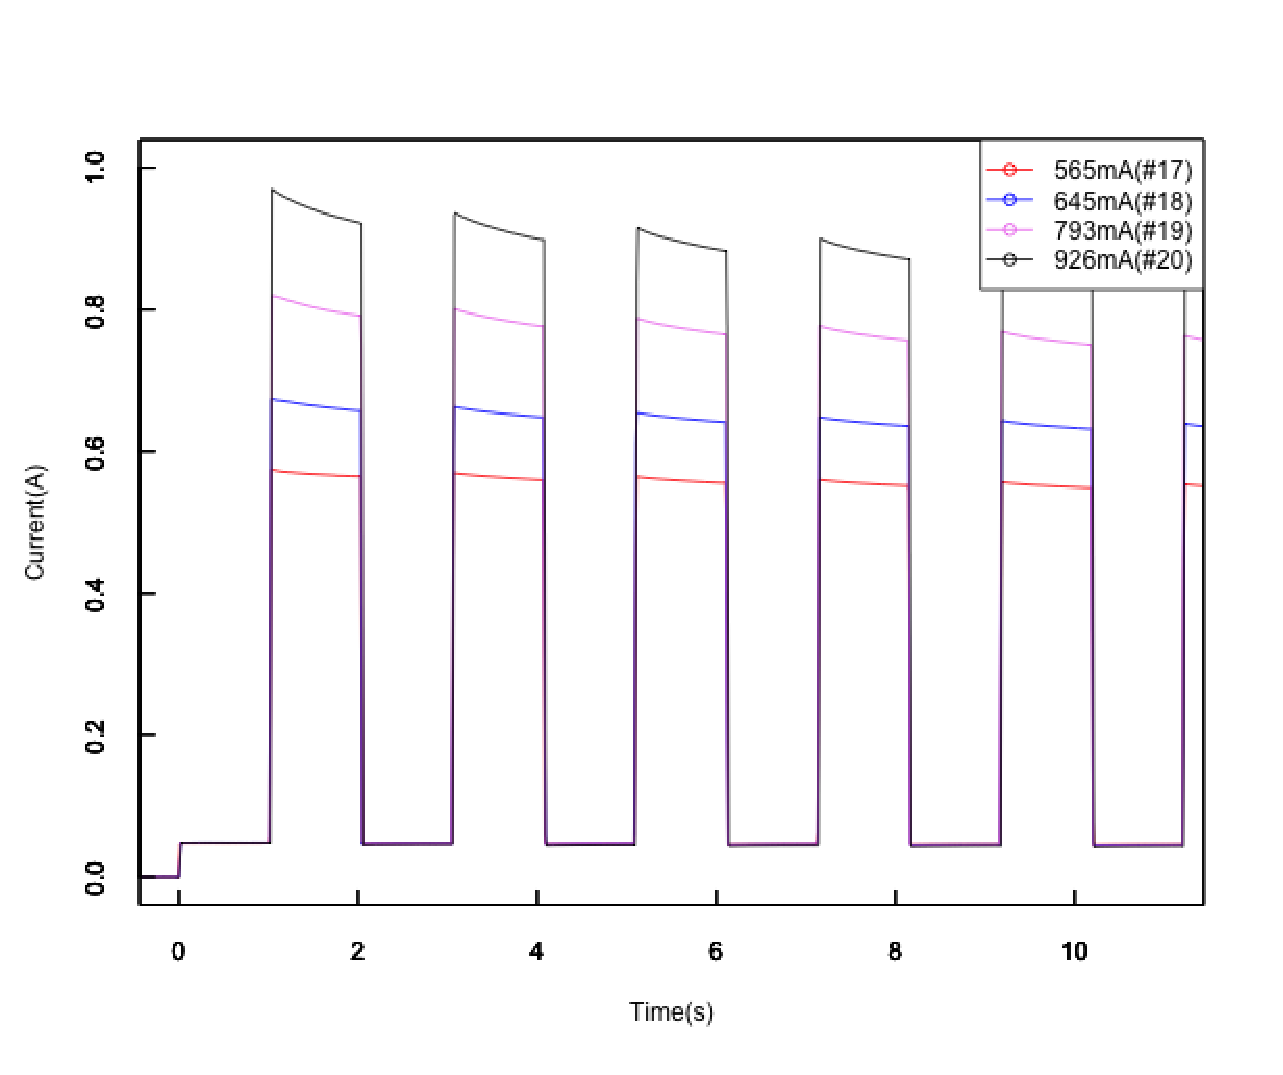
\includegraphics[width=0.9\hsize]{results_discussions/190112_Current_pulse.eps}
  \end{center}
  \caption{}
  \label{fig:190112_Current_pulse}
   \end{minipage}
\end{figure}

パルス印加中とパルス印加前後の試料の顕微鏡写真を図\ref{fig:190112_before_pulse17}から図\ref{fig:190112_after_pulse20}に示す。写真は顕微鏡で撮影した動画から切り取ってきたものである。動画撮影中のセットアップは変化させなかったが、撮影後、相転移が見やすくなるように露出とコントラス、色調を調整した。
\begin{figure}[htbp]
 \begin{minipage}{0.5\hsize}
  \begin{center}
   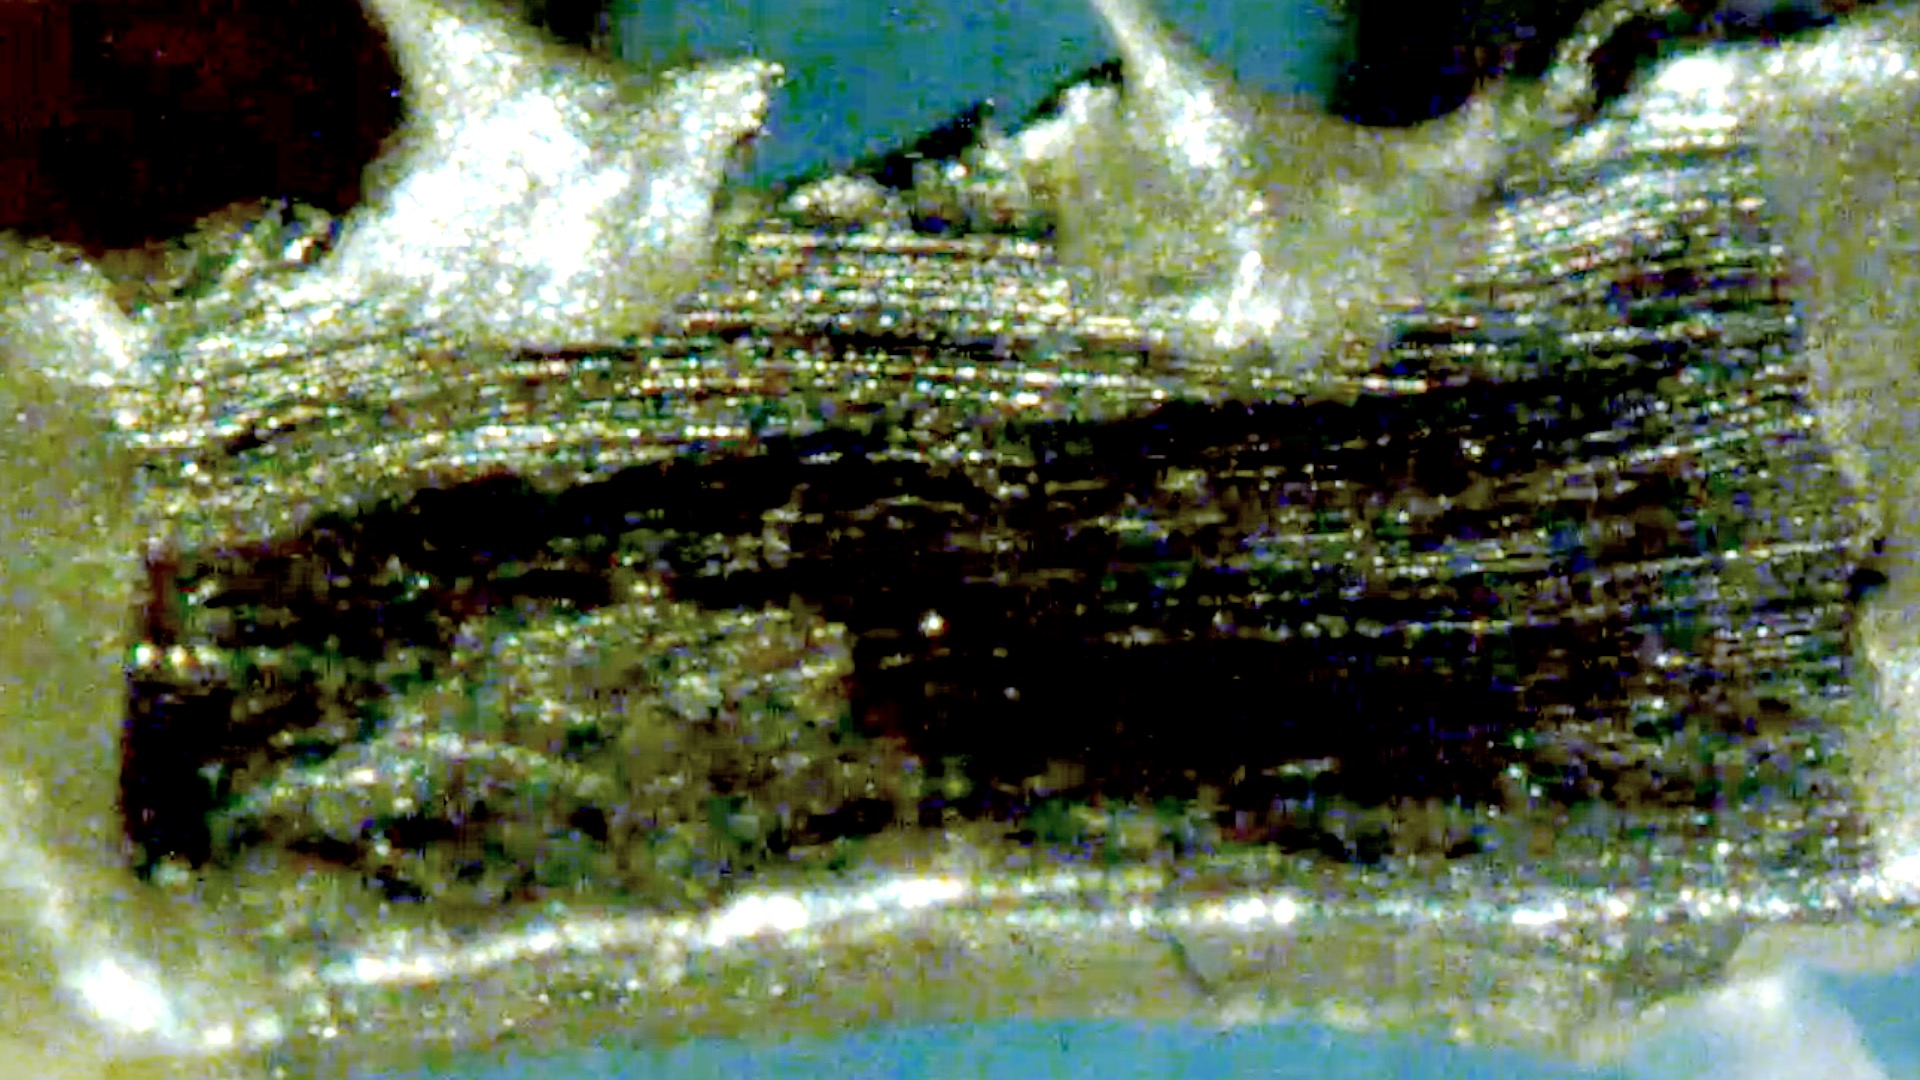
\includegraphics[width=\hsize]{results_discussions/190112_before_pulse17.eps}
  \end{center}
  \caption{}
  \label{fig:190112_before_pulse17}
 \end{minipage}
 \begin{minipage}{0.5\hsize}
  \begin{center}
   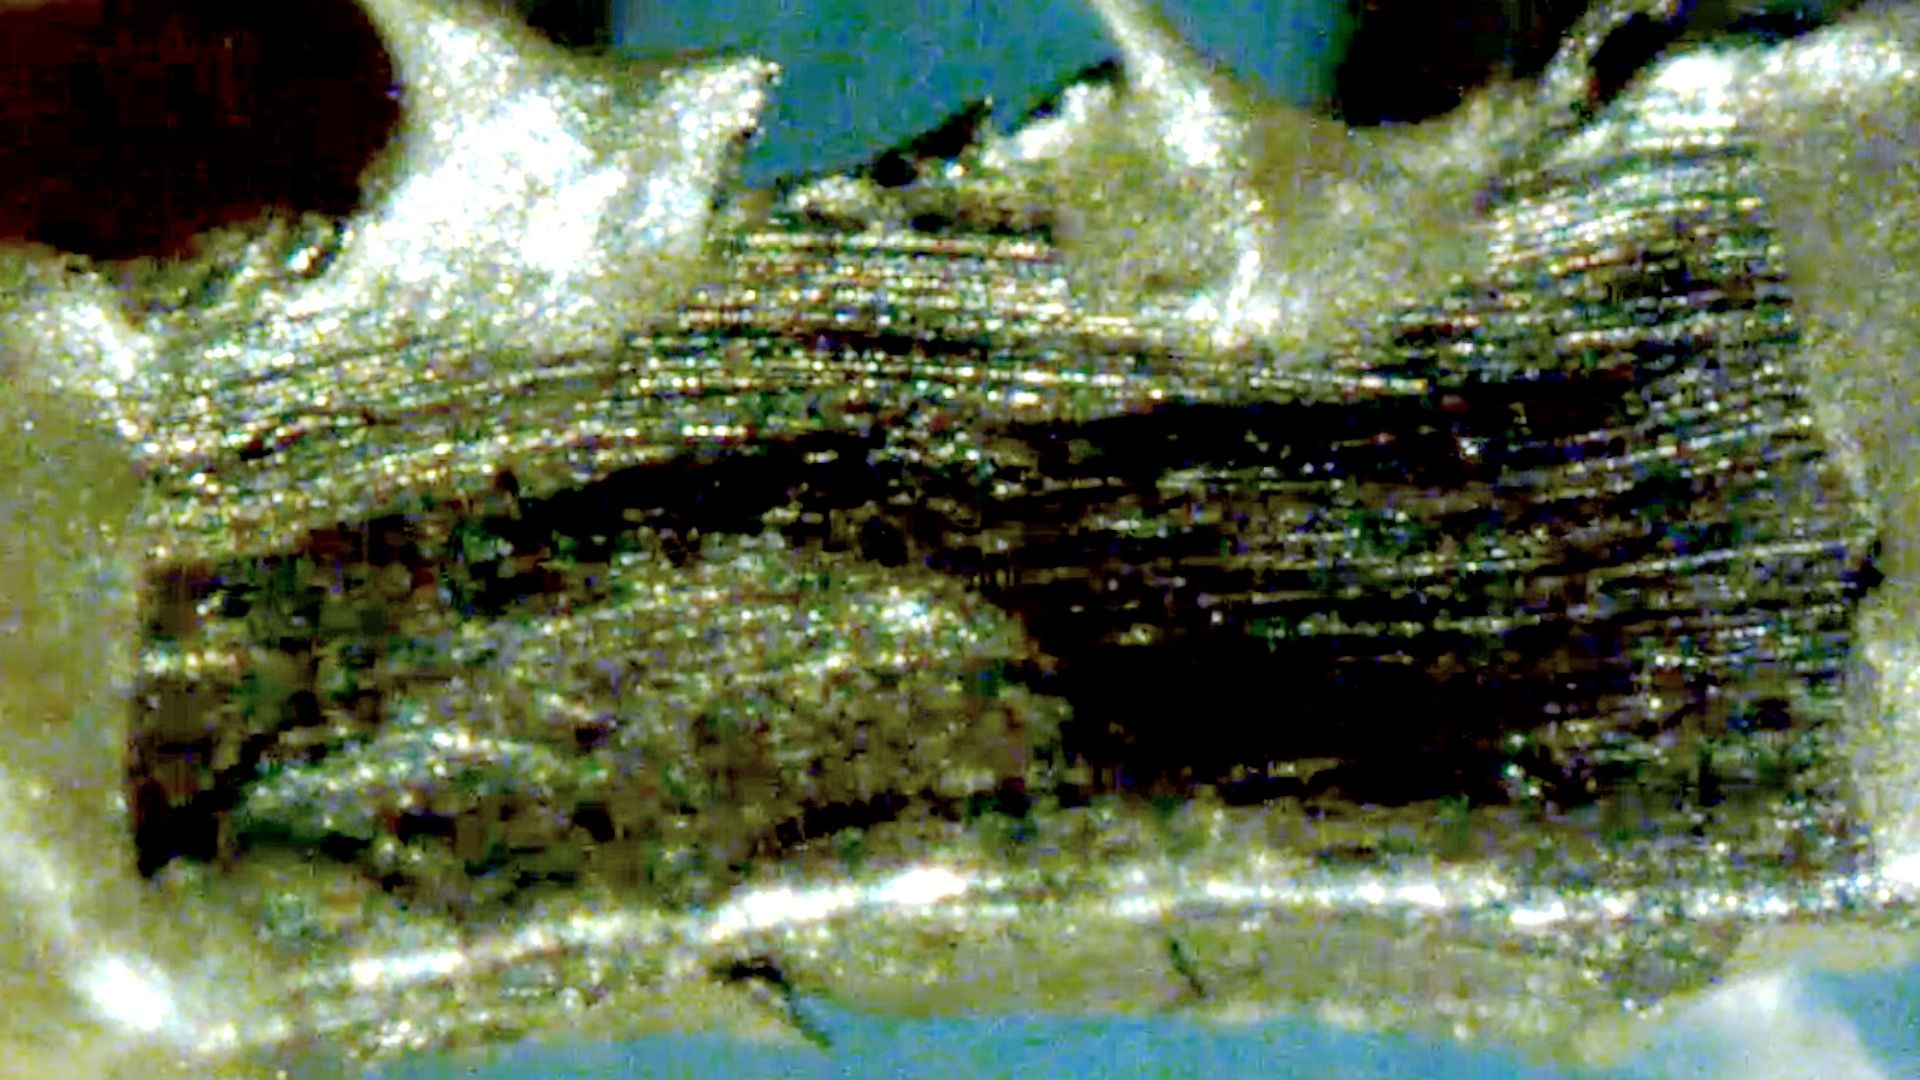
\includegraphics[width=\hsize]{results_discussions/190112_after_pulse17.eps}
  \end{center}
  \caption{}
  \label{fig:190112_after_pulse17}
 \end{minipage}
  \begin{minipage}{0.5\hsize}
  \begin{center}
   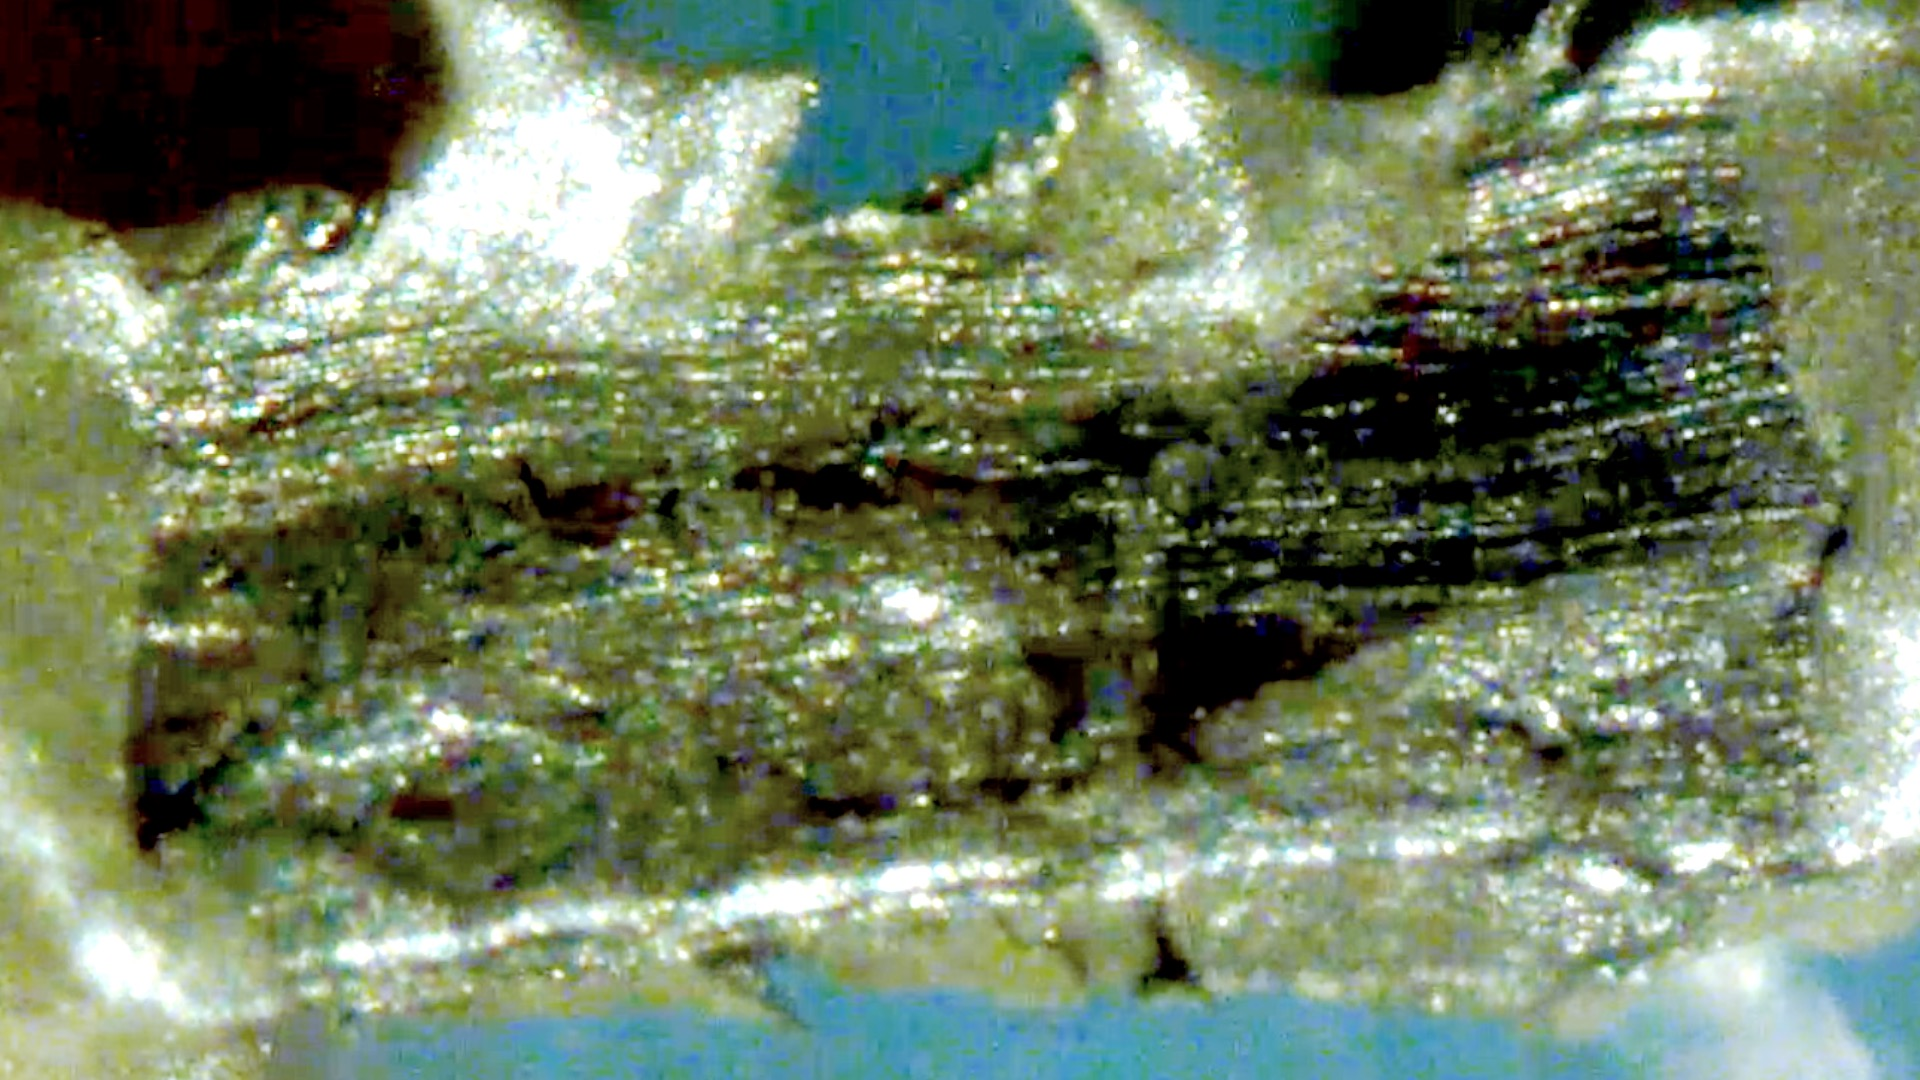
\includegraphics[width=\hsize]{results_discussions/190112_after_pulse19_1.eps}
  \end{center}
  \caption{}
  \label{fig:190112_after_pulse19_1}
 \end{minipage}
  \begin{minipage}{0.5\hsize}
  \begin{center}
   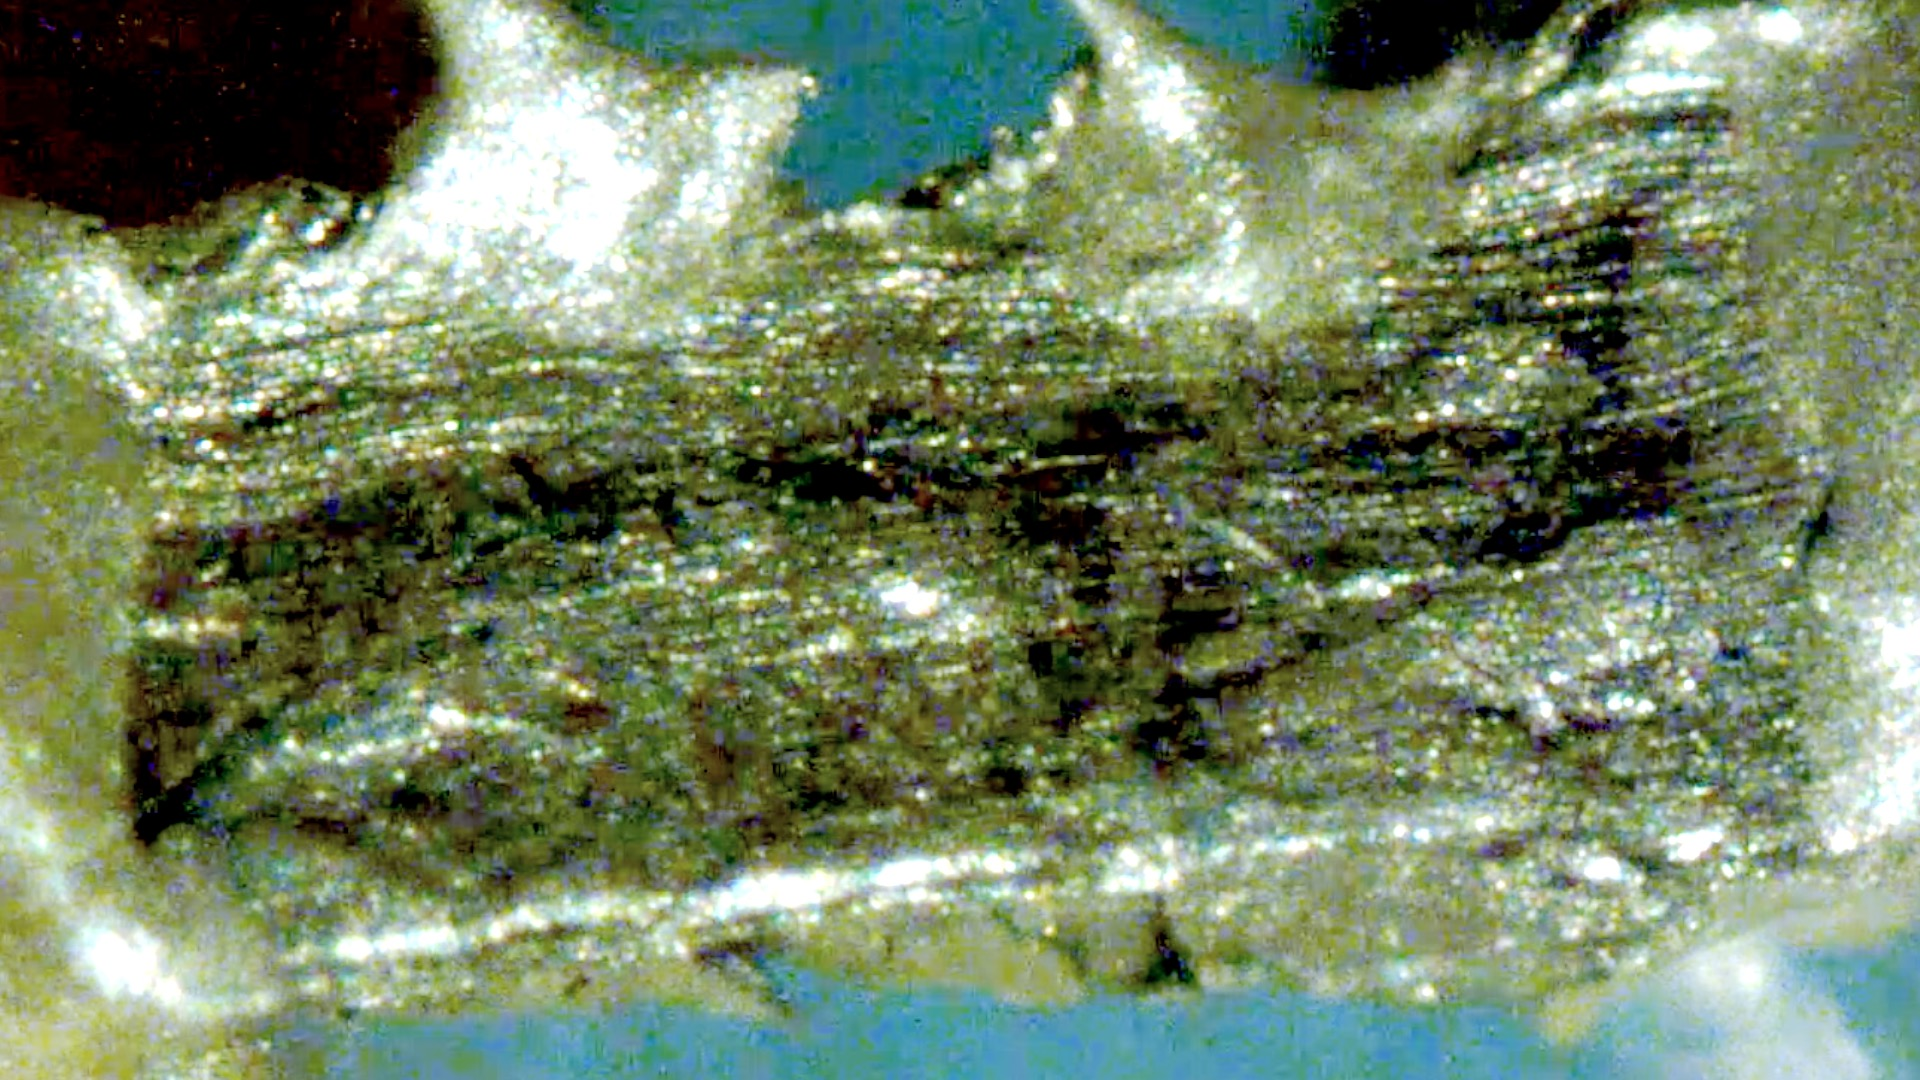
\includegraphics[width=\hsize]{results_discussions/190112_after_pulse19_2.eps}
  \end{center}
  \caption{}
  \label{fig:190112_after_pulse19_2}
 \end{minipage}
  \begin{minipage}{0.5\hsize}
  \begin{center}
   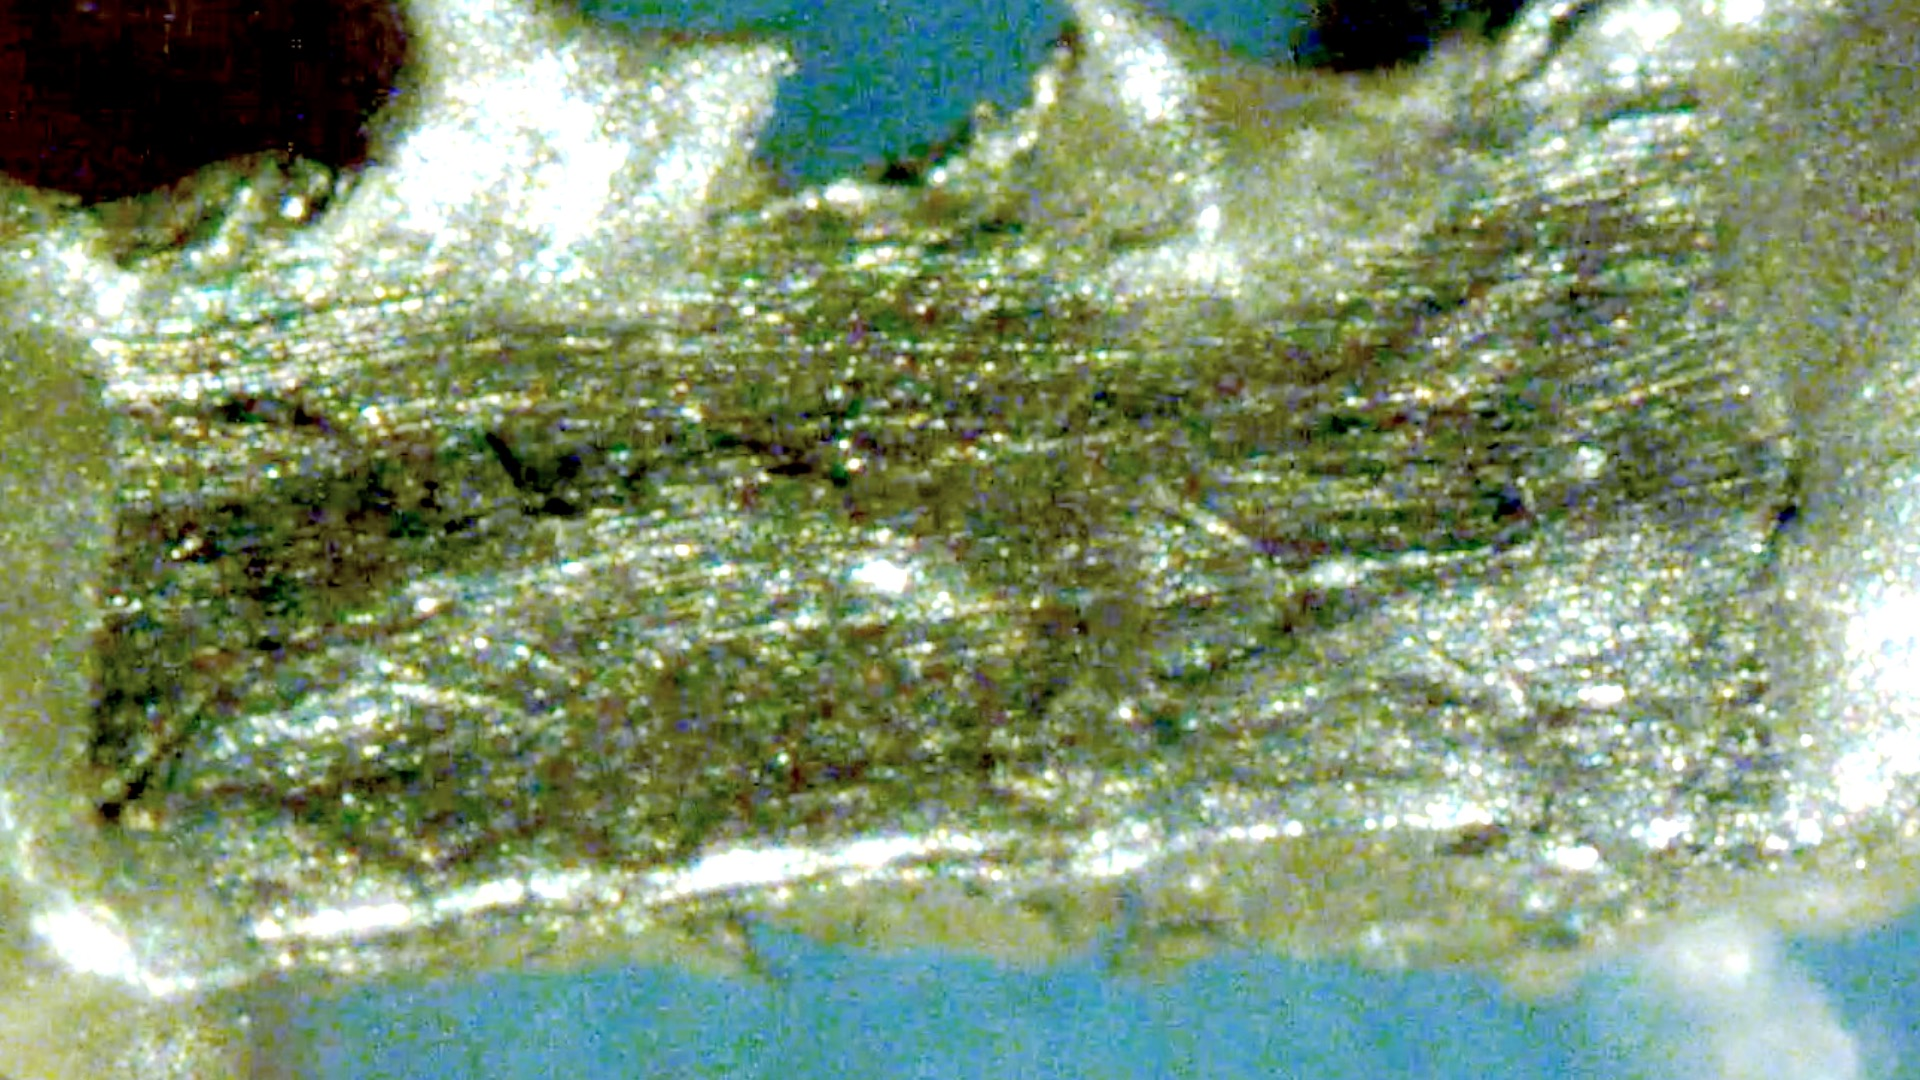
\includegraphics[width=\hsize]{results_discussions/190112_after_pulse20.eps}
  \end{center}
  \caption{}
  \label{fig:190112_after_pulse20}
 \end{minipage}
\end{figure}
No.17のパルス列を印加する前の画像(図\ref{fig:190112_before_pulse17})と全てのパルスを印加した後の画像(図\ref{fig:190112_after_pulse20})を比較すると、黒色の半導体的な吸収を示すαスズから金属的な光沢を持つβスズへの転移がはっきりと見て取れる。また詳しく見ると、相転移は熱の流入源である左側の電流端子から始まり、熱の流出先である二つの電圧端子と右側の電流端子に向かって進行していることがわかる。


\begin{figure}[!h]
 \begin{minipage}{\hsize}
    \begin{center}
   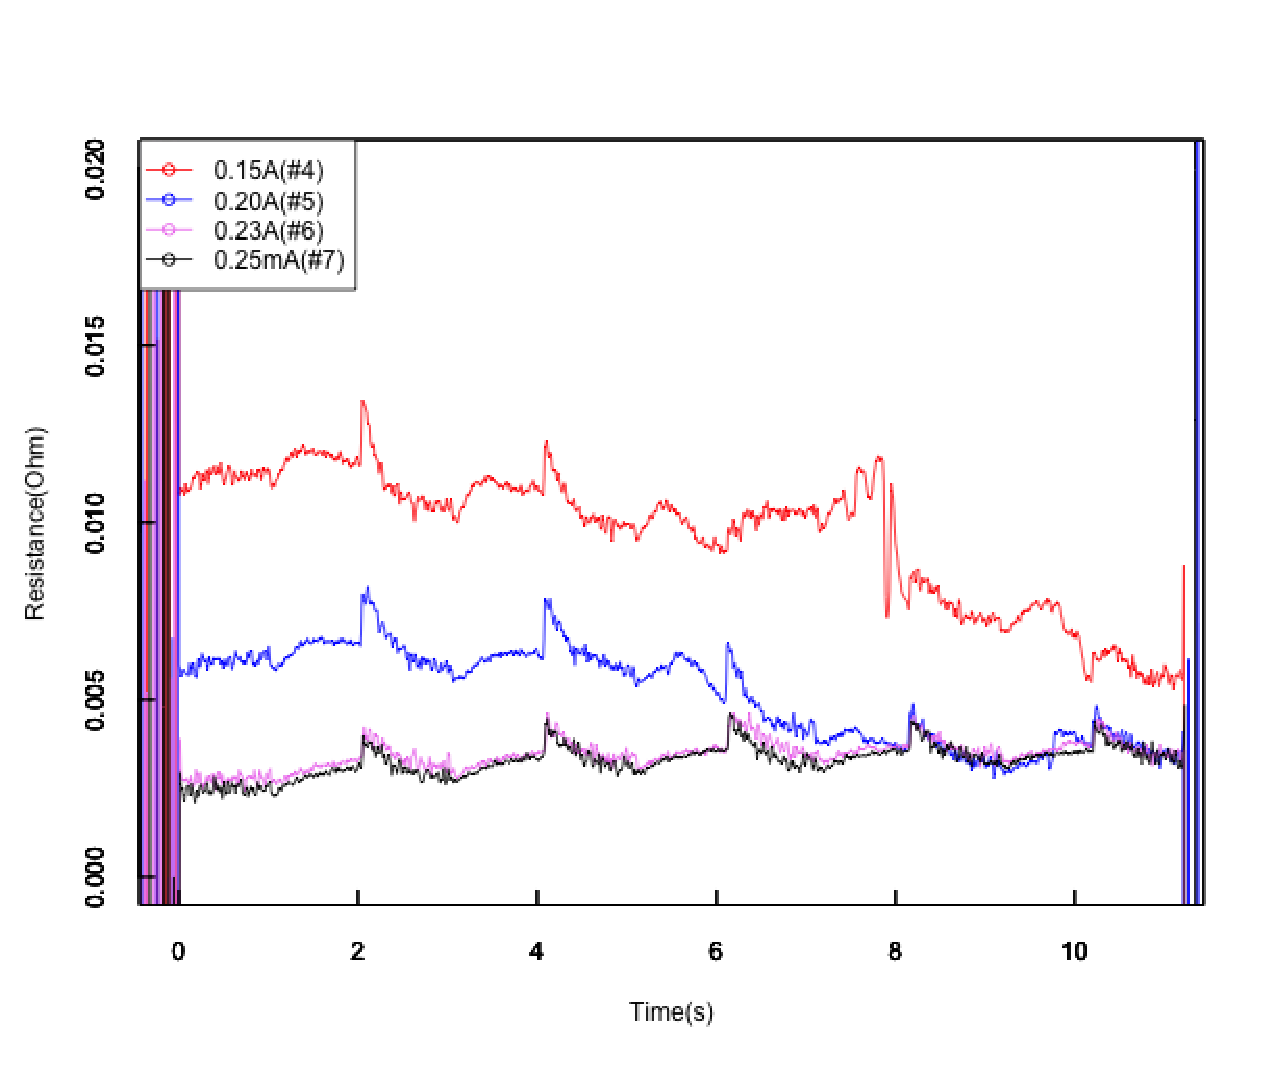
\includegraphics[width=0.9\hsize]{results_discussions/190113_Resistance_pulse.eps}
  \end{center}
  \caption{}
  \label{fig:190113_Resistance_pulse}
 \end{minipage}
 \begin{minipage}{\hsize}
     \begin{center}
   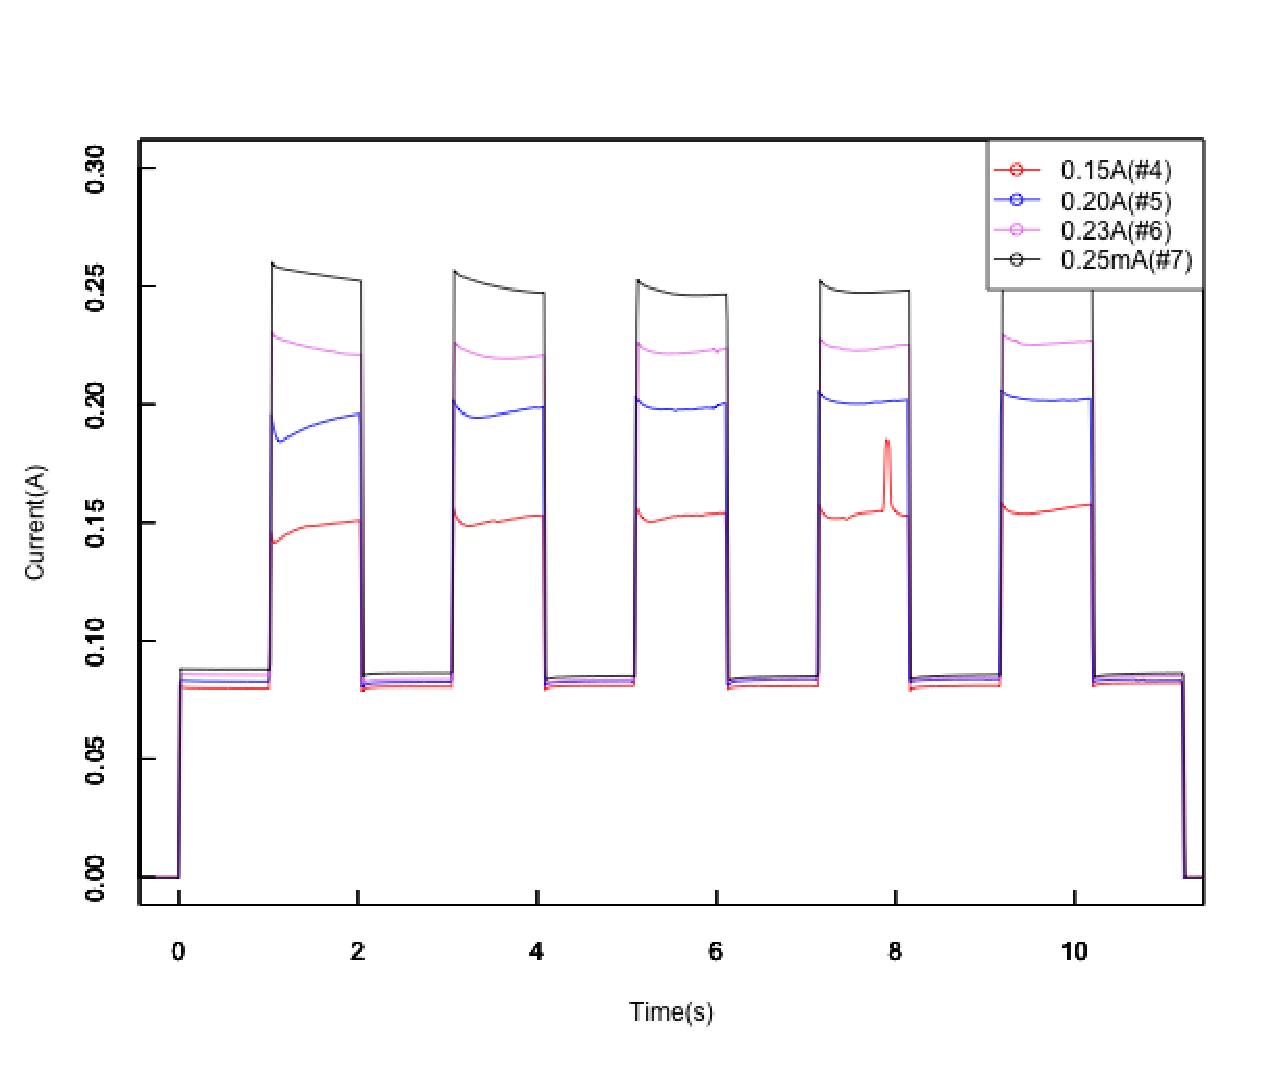
\includegraphics[width=0.9\hsize]{results_discussions/190113_Current_pulse.eps}
  \end{center}
  \caption{}
  \label{fig:190113_Current_pulse}
   \end{minipage}
\end{figure}

\begin{figure}[htbp]
 \begin{minipage}{0.5\hsize}
  \begin{center}
   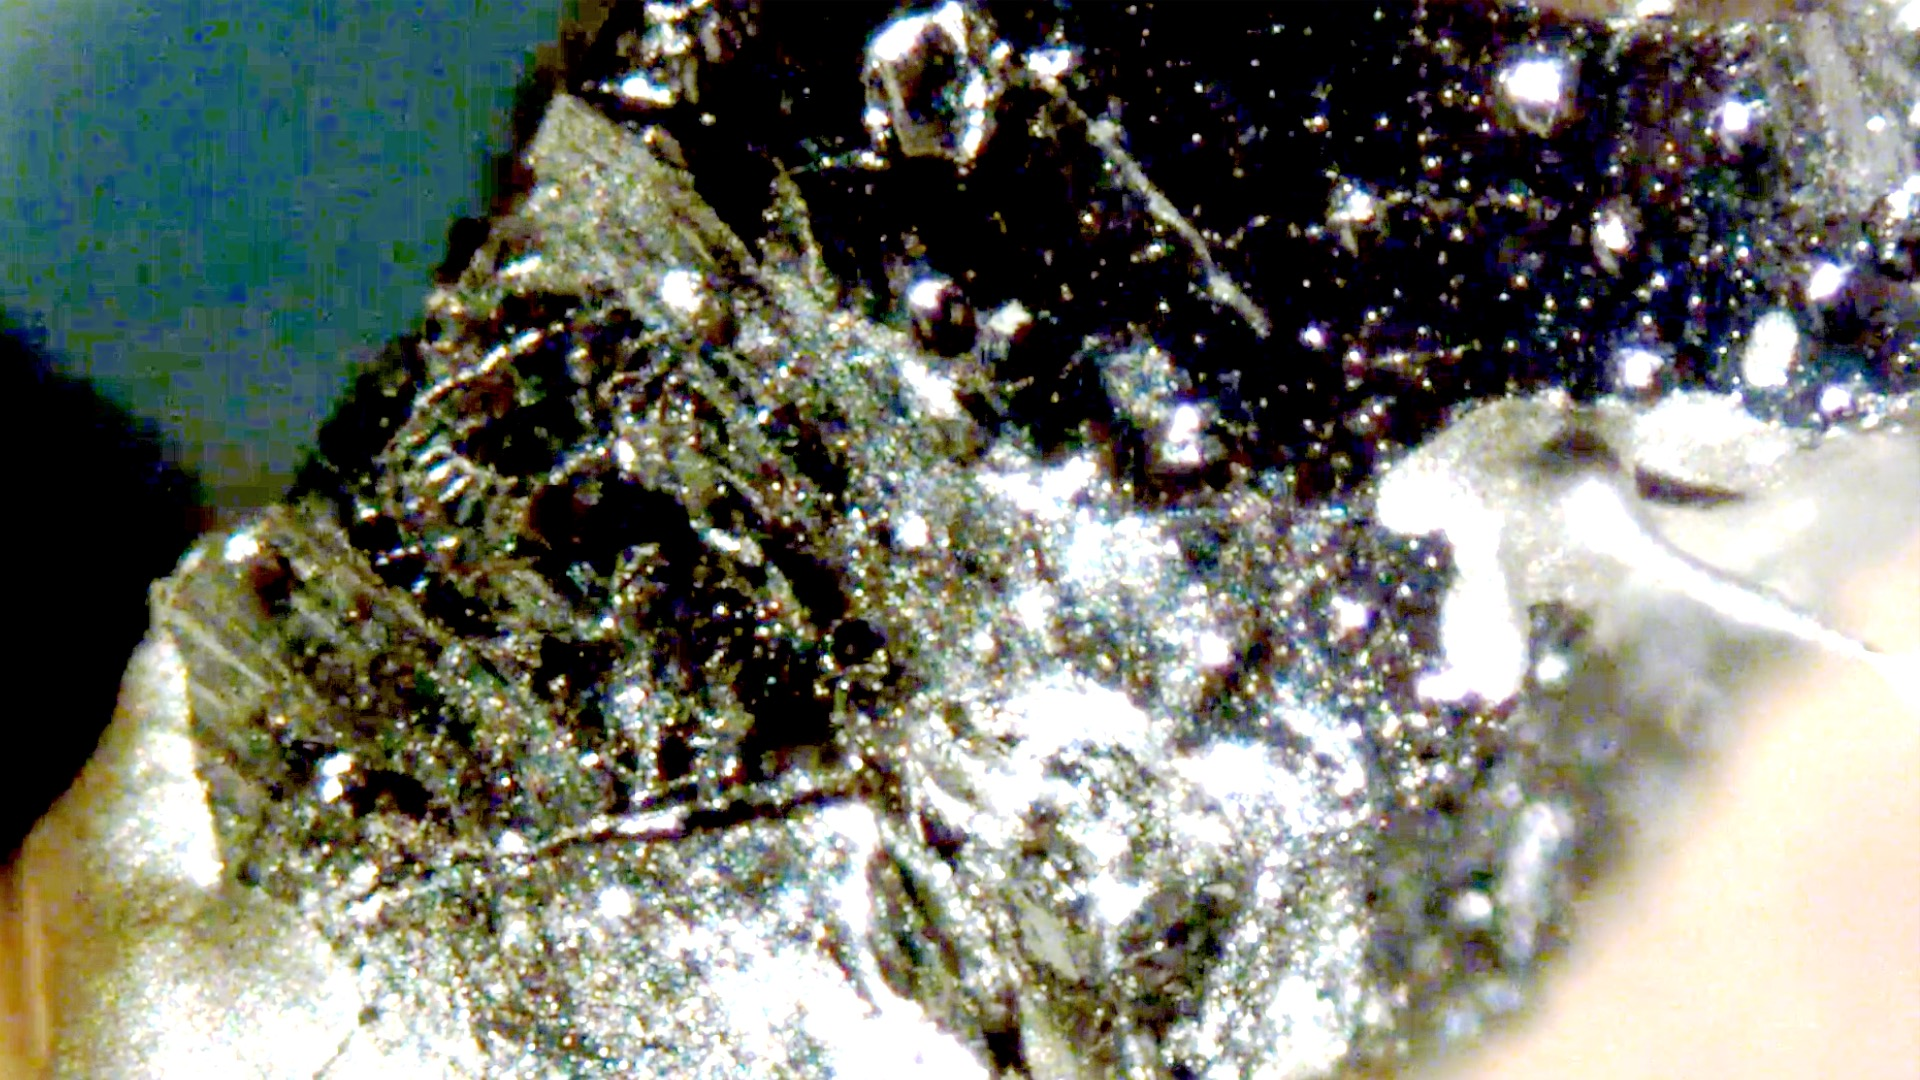
\includegraphics[width=\hsize]{results_discussions/190113_before_pulse5.eps}
  \end{center}
  \caption{}
  \label{fig:190113_before_pulse5}
 \end{minipage}
 \begin{minipage}{0.5\hsize}
  \begin{center}
   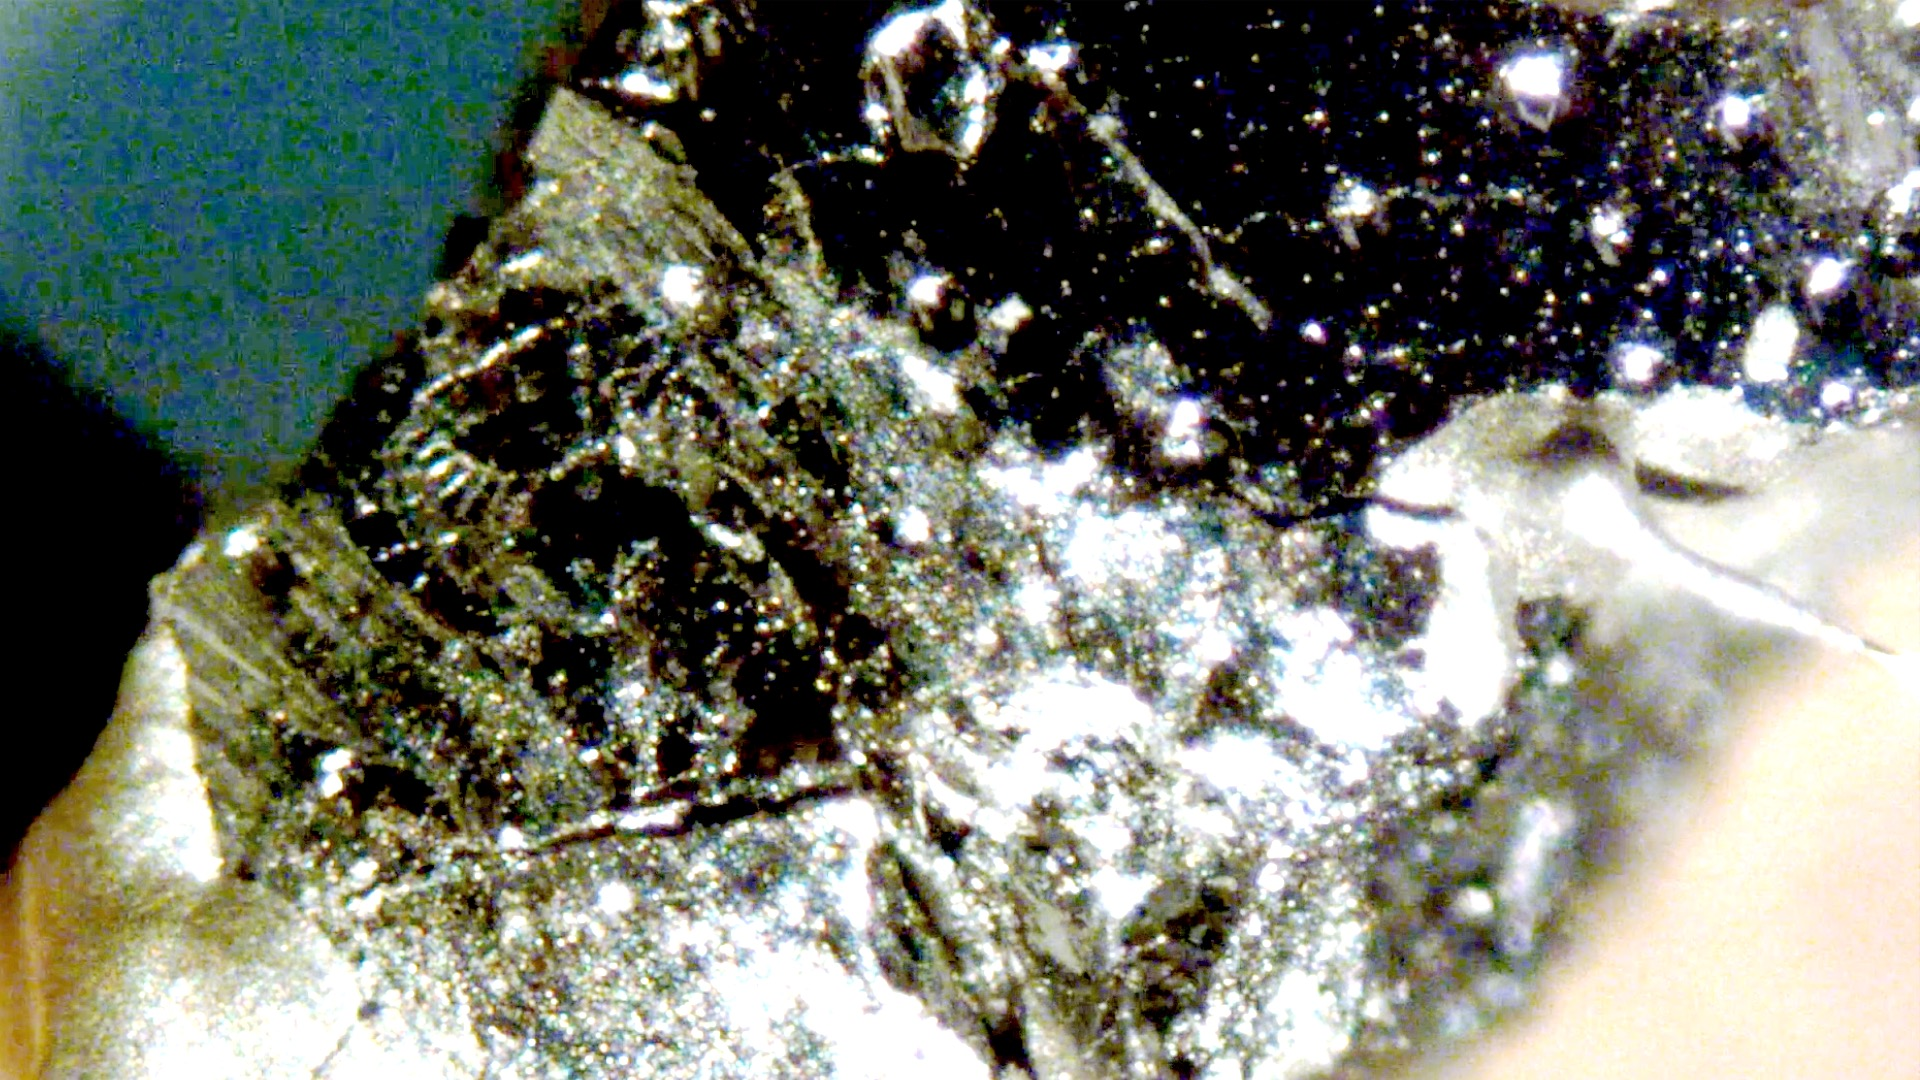
\includegraphics[width=\hsize]{results_discussions/190113_after_pulse5-1.eps}
  \end{center}
  \caption{}
  \label{fig:190113_after_pulse5-1}
 \end{minipage}
  \begin{minipage}{0.5\hsize}
  \begin{center}
   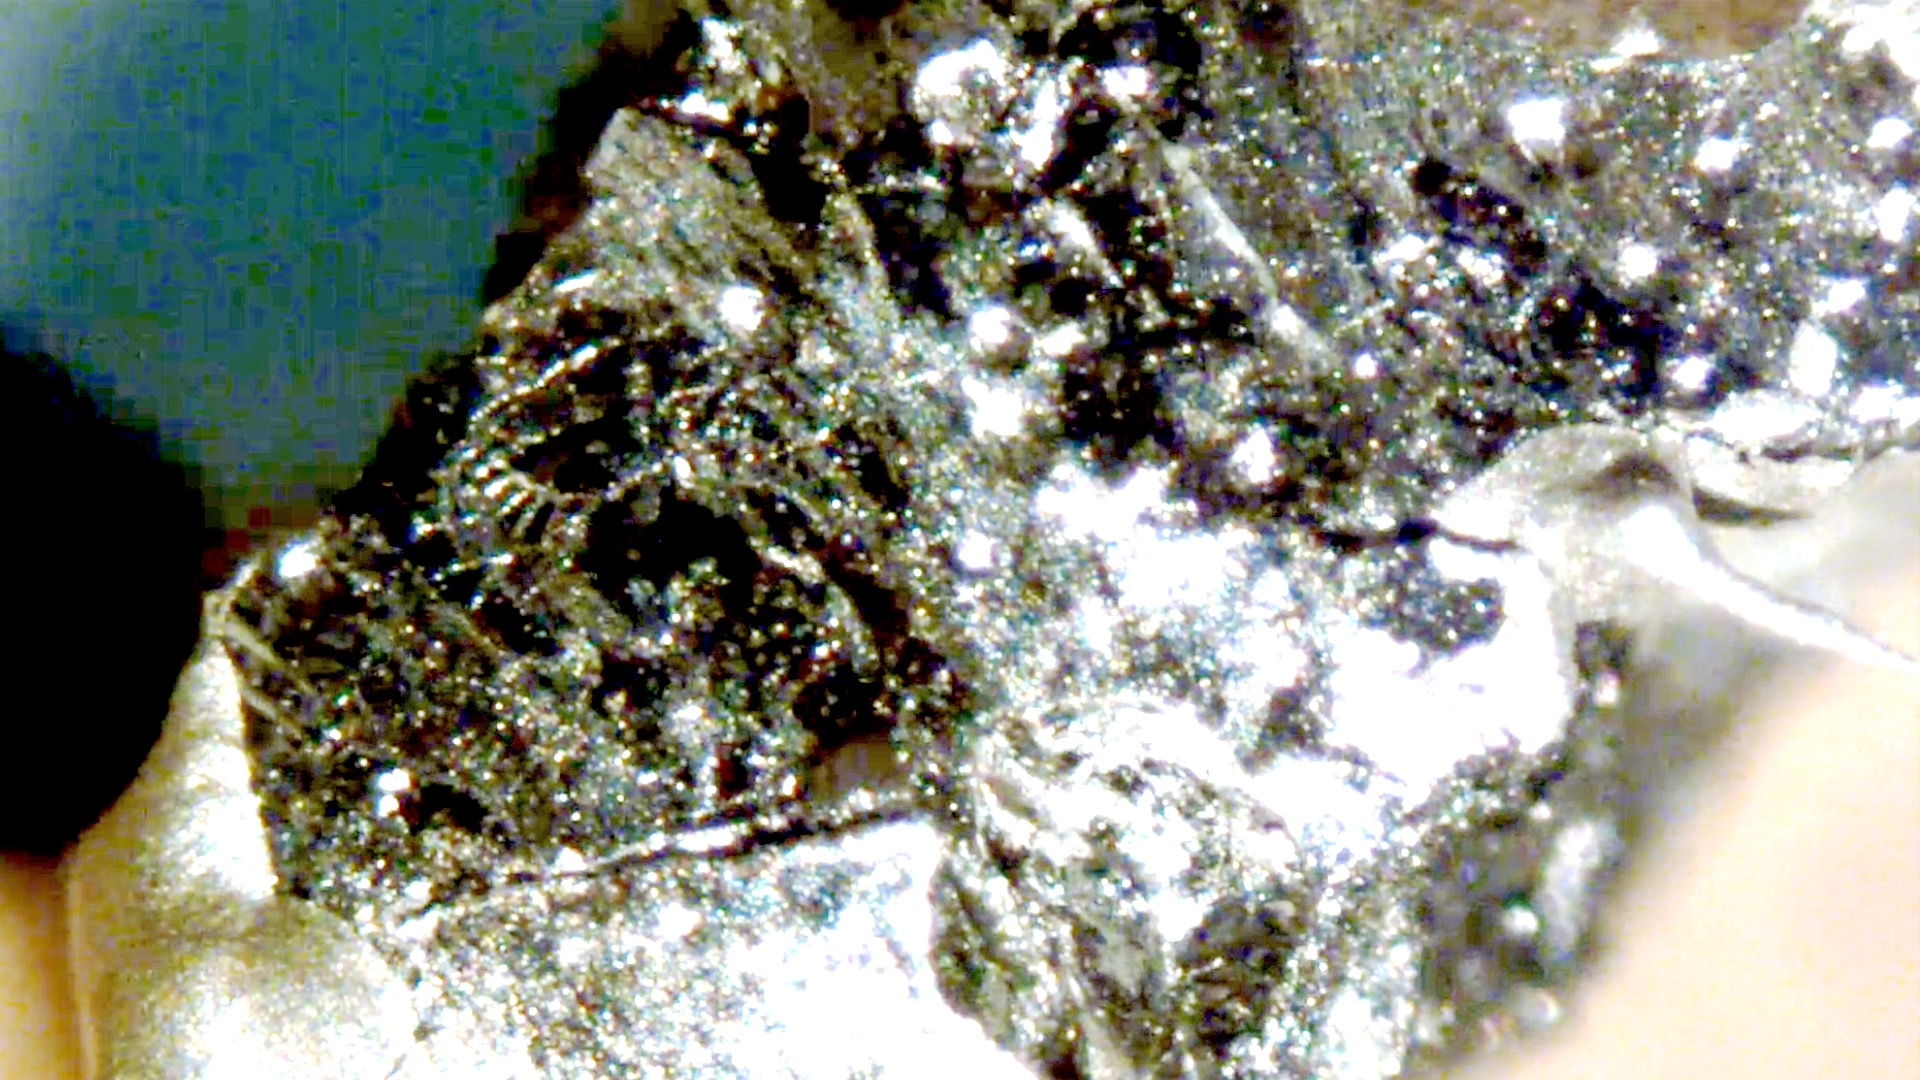
\includegraphics[width=\hsize]{results_discussions/190113_after_pulse5-2.eps}
  \end{center}
  \caption{}
  \label{fig:190113_after_pulse5-2}
 \end{minipage}
  \begin{minipage}{0.5\hsize}
  \begin{center}
   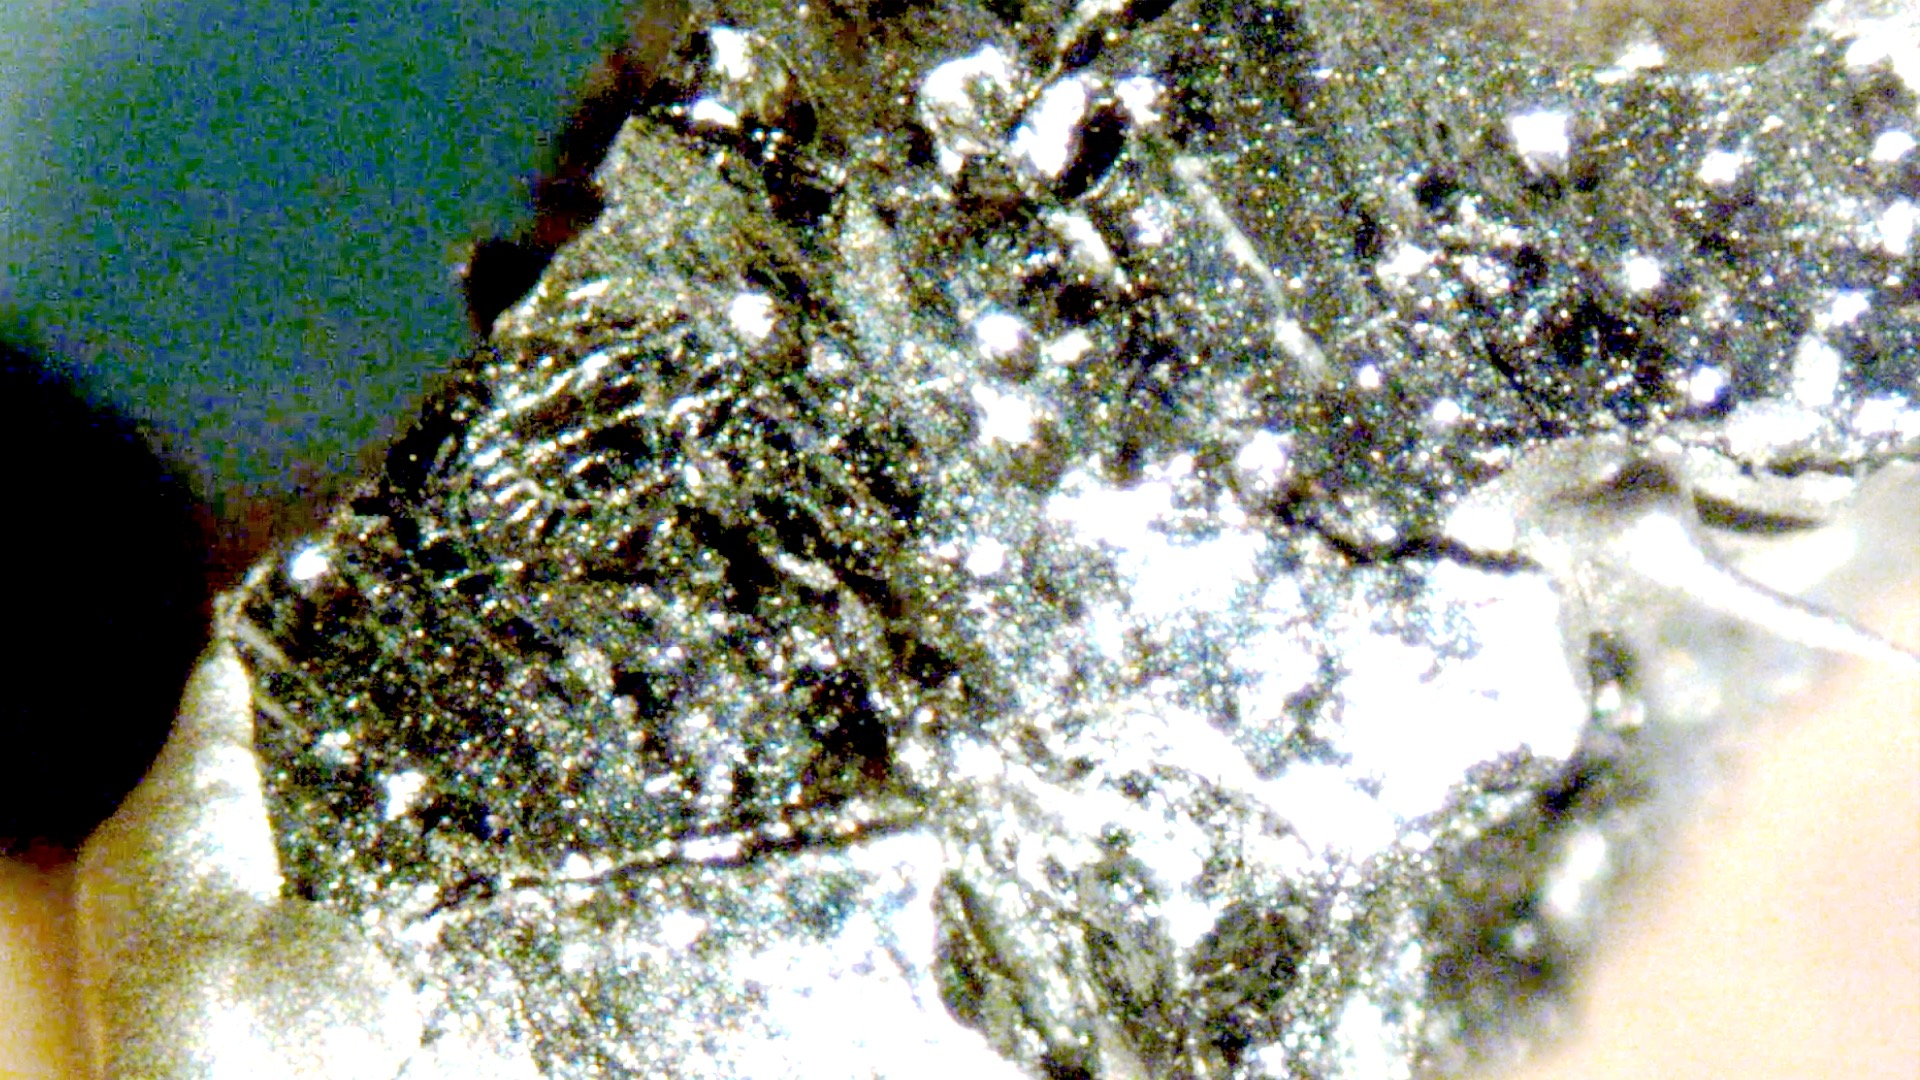
\includegraphics[width=\hsize]{results_discussions/190113_after_pulse5-3.eps}
  \end{center}
  \caption{}
  \label{fig:190113_after_pulse5-3}
 \end{minipage}
  \begin{minipage}{0.5\hsize}
  \begin{center}
   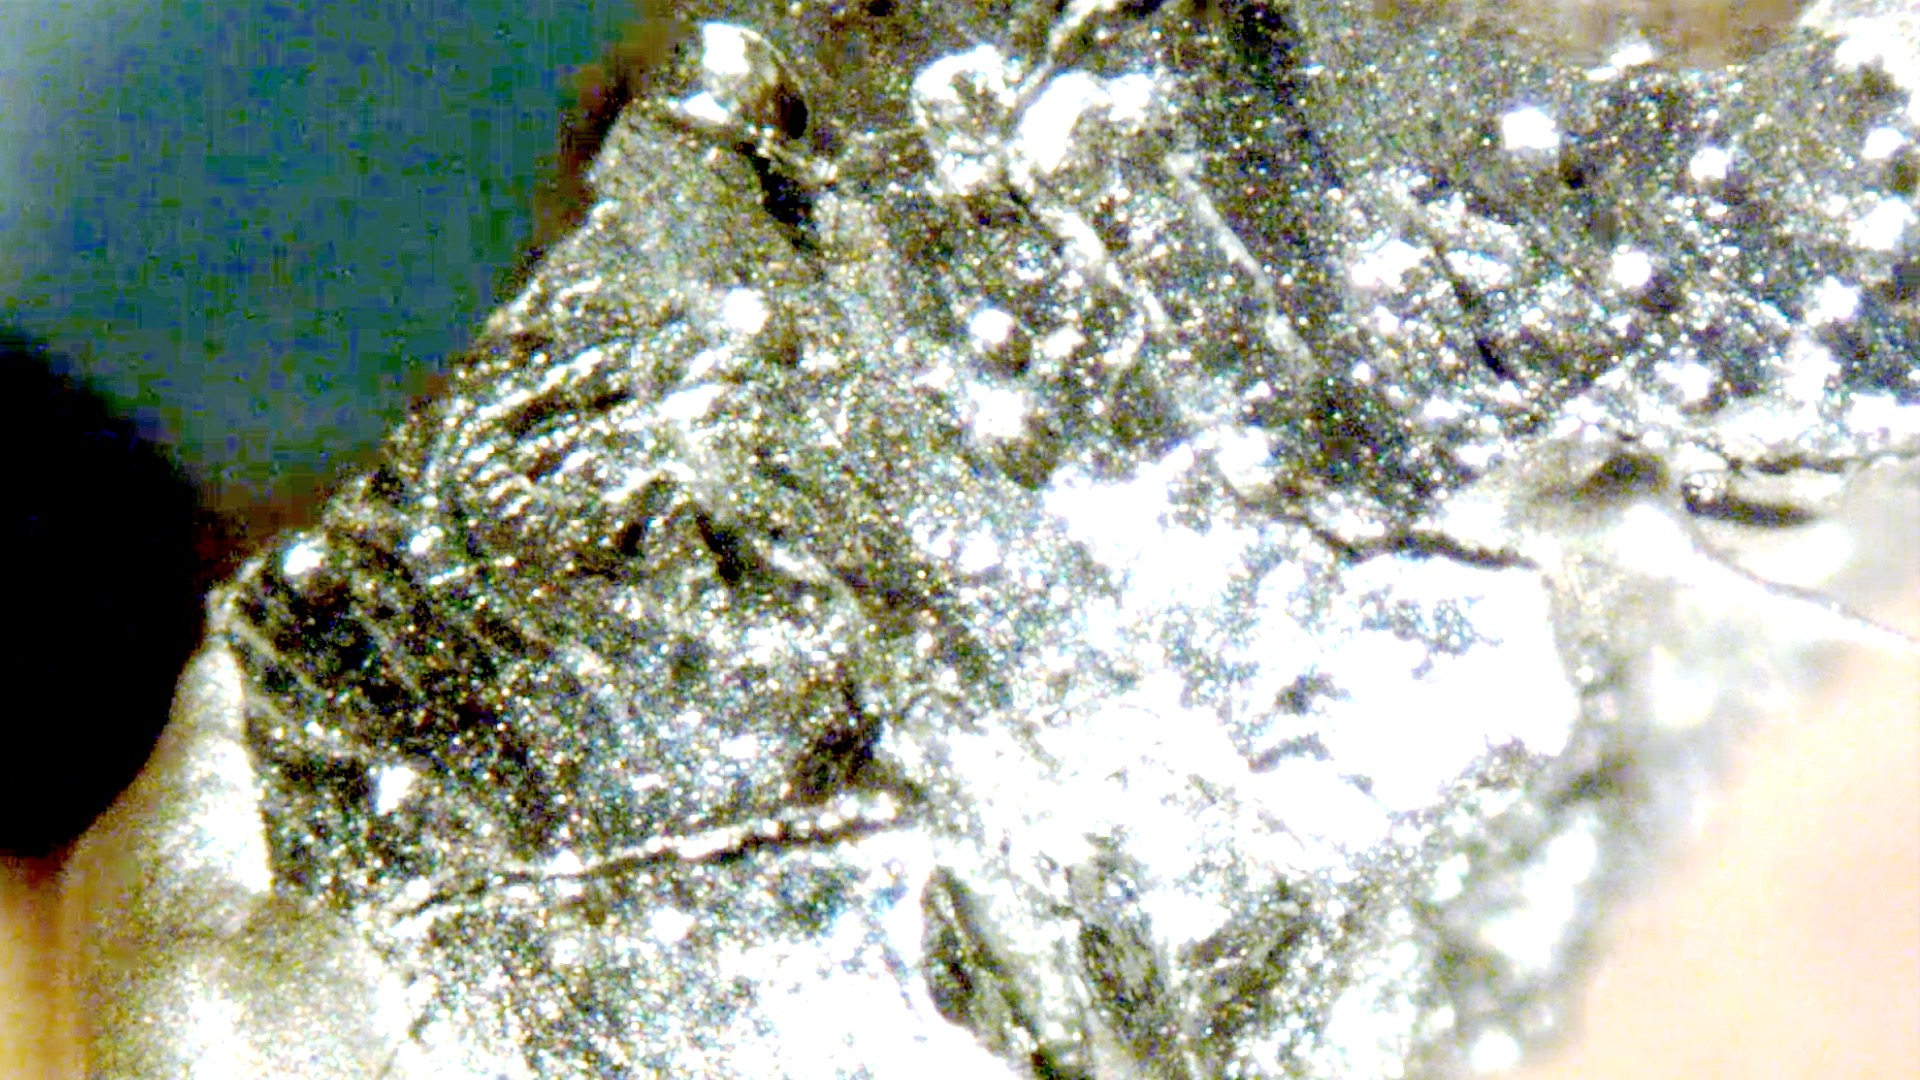
\includegraphics[width=\hsize]{results_discussions/190113_after_pulse6.eps}
  \end{center}
  \caption{}
  \label{fig:190113_after_pulse6}
 \end{minipage}
\end{figure}


%\subsection{電流パルスを用いたβ相からα相への変換}

\clearpage

%cd Documents/GitManagedProjects-Kagawalab/報告書/卒業論文/results_discussions/